\chapter{Utero-placental pump} \label{sec:contractions}
    \todoitemtwo{2024-05-03 RO: Simplify discussion of results in this chapter.}
    \todoitemthree{For viva: What is $\mathcal{H}$? And $\alpha$?}

    In \citeyear{dellschaftHaemodynamicsHumanPlacenta2020}, \citeauthor{dellschaftHaemodynamicsHumanPlacenta2020} \cite{dellschaftHaemodynamicsHumanPlacenta2020} were the first to report the so-called `utero-placental pump' phenomenon. The utero-placental pump is a type of placental contraction that involves only the placenta, and is therefore unlike previously documented Braxton-Hicks that involves contractions of the entire uterus \cite{togashiSustainedUterineContractions1993}.

    Here, we will outline a preliminary model of the utero-placental pump, utilising the same blood flow model, oxygen transport model, and placenta geometry from Chapter \ref{sec:modelling}. We impose boundary motion as a first step to understand how shape change during the utero-placental pump influences oxygen transport, rather than model the mechanism of the contractions. This work uses a prescribed so-called `domain velocity', which specifies how the domain should evolve; we will use the domain velocity through methods known as moving mesh methods, which specify how the discretisation handles the domain movement. As far as we are aware, this is the first model of maternal blood flow that considers the utero-placental pump, and lays the computational framework for understanding oxygen transport and placental disease during these contractions.
    
    In \S\ref{sec:contractions:dgfem-discretisation}, we will begin by introducing a modified DGFEM scheme that is valid for time-dependent domains $\Omega(t)$. \S\ref{sec:contractions:numerical-experiments} will then present some basic numerical experiments that show optimal convergence rates under spatial mesh and time-step refinement, and show how NSD (Navier-Stokes-Darcy) behaves with solid boundary movement. \S\ref{sec:contractions:placenta} will provide the main results of this chapter, with domain movement applied to the asymmetric placenta problem originally presented in \S\ref{sec:numerical-methods:blood-flow-experiments:asymmetric}. \S\ref{sec:contractions:summary} will conclude with an overview of the results and future work.

    \section{DGFEM discretisations} \label{sec:contractions:dgfem-discretisation}    
        We will first derive finite element methods for moving domains, where each point in the domain evolves according to domain velocity $\vec{w}(\vec{x}, t)$. We start by taking a general scalar time-dependent PDE problem: find $u$ such that
        \begin{equation}
            \pdv{u}{t} = \mathcal{L} u,
            \label{eq:general-scalar-problem}
        \end{equation}
        where $\mathcal{L}$ is some spatial differential operator. As is typical for deriving finite element methods, we multiply Equation \eqref{eq:general-scalar-problem} by an appropriate test function and integrate to give:
        \begin{equation}
            \int_\Omega \pdv{u}{t} v \diff \vec{x} = \int_\Omega (\mathcal{L} u) v \diff \vec{x}.
            \label{eq:general-scalar-problem-mult-and-int}
        \end{equation}
        We next state the Reynolds Transport Theorem from \citeauthor{arisVectorsTensorsBasic1989} \cite{arisVectorsTensorsBasic1989}.
        \begin{theorem}
            Let $\Omega(t)$ be a time-dependent closed domain for $t \in [0, T]$, with points moving continuously according to domain velocity $\vec{w}(\vec{x}, t) \equiv \dv{\vec{x}}{t}$ in $\Omega(t)$, and $\mathcal{F}(\vec{x}, t)$ be any scalar function. Then
            \begin{equation}
                \dv{}{t} \int_{\Omega(t)} \mathcal{F} \diff\vec{x} = \int_{\Omega(t)} \pdv{\mathcal{F}}{t} \diff\vec{x} + \int_{\partial\Omega(t)} \mathcal{F} (\vec{w} \cdot \vec{n}) \diff s,
                \label{eq:reynolds-transport-theorem}    
            \end{equation}
            where $\vec{n}(t)$ denotes the outward unit normal to $\Omega(t)$, and $\partial\Omega(t)$ is the closed surface forming the boundary of $\Omega(t)$.
        \end{theorem}
        \begin{proof}
            Proof can be found in \citeauthor{arisVectorsTensorsBasic1989} \cite{arisVectorsTensorsBasic1989}.
        \end{proof}\noindent
        Using Equation \eqref{eq:reynolds-transport-theorem} with $\mathcal{F} = uv$ in combination with the product rule, the LHS of Equation \eqref{eq:general-scalar-problem-mult-and-int} can be written as
        \begin{equation}
            \dv{}{t} \int_{\Omega(t)} uv \diff\vec{x} - \int_{\Omega(t)} u\pdv{v}{t} \diff\vec{x} - \int_{\partial\Omega(t)} uv (\vec{w} \cdot \vec{n}) \diff s = \int_\Omega \pdv{u}{t} v \diff \vec{x}.
            \label{mm-derivation:1}
        \end{equation}
        We next state the divergence theorem from \citeauthor{matthewsVectorCalculus} \cite{matthewsVectorCalculus}.
        \begin{theorem}
            Let $\vec{\mathcal{G}}$ be a continuously differentiable vector field defined in $\Omega$. Then
            \begin{equation}
                \int_{\Omega} \vec{\nabla} \cdot \vec{\mathcal{G}} \diff\vec{x} = \int_{\partial\Omega} \vec{\mathcal{G}} \cdot \vec{n} \diff s,
                \label{eq:divergence-theorem}
            \end{equation}
            where $\vec{n}$ denotes the outward unit normal to $\Omega$, and $\partial\Omega$ is the closed surface forming the boundary of $\Omega$.
        \end{theorem}
        \begin{proof}
            Proof can be found in \citeauthor{matthewsVectorCalculus} \cite{matthewsVectorCalculus}.
        \end{proof}\noindent
        Using Equation \eqref{eq:divergence-theorem} with $\vec{\mathcal{G}} = uv\vec{w}$ in combination with the product rule, Equation \eqref{mm-derivation:1} can be written as
        \begin{equation}
            \dv{}{t} \int_{\Omega(t)} uv \diff\vec{x} - \int_{\Omega(t)} \left( u\pdv{v}{t} + u(\vec{w} \cdot \vec{\nabla}v) + \vec{\nabla} \cdot (u \vec{w}) v \right) \diff \vec{x} = \int_\Omega \pdv{u}{t} v \diff \vec{x}.
            \label{mm-derivation:2}
        \end{equation}
        We assume that the test functions move with the domain velocity, which is a valid assumption for simplex meshes with flat faces \cite{nobileStabilityAnalysisArbitrary1999}:
        \begin{equation*}
            \pdv{v}{t} + \vec{w} \cdot \vec{\nabla}v = 0.
        \end{equation*}
        This allows us to write Equation \eqref{mm-derivation:2} as
        \begin{equation}
            \dv{}{t} \int_{\Omega(t)} uv \diff\vec{x} - \int_{\Omega(t)} \vec{\nabla} \cdot (u\vec{w}) v \diff \vec{x} = \int_\Omega \pdv{u}{t} v \diff \vec{x}.
            \label{eq:moving-mesh-relation-scalar}
        \end{equation}
        For the equivalent vector problem, i.e.,
        \begin{equation}
            \pdv{\vec{u}}{t} = \mathcal{L} \vec{u},
        \end{equation}
        with test functions $\vec{v}$, this relation is
        \begin{equation}
            \dv{}{t} \int_{\Omega(t)} \vec{u} \cdot \vec{v} \diff\vec{x} - \int_{\Omega(t)} [\vec{\nabla} \cdot (\vec{u} \otimes \vec{w})] \cdot \vec{v} \diff \vec{x} = \int_\Omega \pdv{\vec{u}}{t} \cdot \vec{v} \diff \vec{x}.
            \label{eq:moving-mesh-relation}
        \end{equation} \noindent

        \subsection{Navier-Stokes-Darcy discretisation} \label{sec:contractions:dgfem-discretisation:nsd}
            We recall that the NSD equations describing the blood flow in Chapter \ref{sec:modelling} were given by
            \begin{subequations}
                \begin{align} \retag{eq:nsb:momentum}
                    \begin{split}
                        \rho \pdv{\vec{u}}{t} + \Psi \frac{\mu}{k} \vec{u} + \rho (\vec{u} \cdot \vec{\nabla}) \vec{u} - \mu \nabla^2 \vec{u} + \vec{\nabla} p = \vec{f}_\text{f} &~ \text{in } \Omega,
                    \end{split}\\ \retag{eq:nsb:incompressibility}
                    \begin{split}
                        \vec{\nabla} \cdot \vec{u} = 0 &~ \text{in } \Omega.
                    \end{split}%
                \end{align}%
            \end{subequations}%
            The weak formulation for this problem is given by: find $\vec{u}, p$ such that
            \begin{multline}
                \overbrace{L_\text{f}(\vec{u}, \vec{v})}^{\text{time}} + \overbrace{A_\text{f}(\vec{u}, \vec{v})}^{\text{diffusion}} + \overbrace{C_\text{f}(\vec{u}, \vec{v})}^{\text{advection}} + \overbrace{M_\text{f}(\vec{u}, \vec{v})}^{\text{reaction}} + \overbrace{B_\text{f}(\vec{v}, p)}^{\text{pressure}} - \overbrace{B_\text{f}(\vec{u}, q)}^{\text{incompressibility}} \\ = \overbrace{F_{\text{f},\vec{g}_\text{f,D},\vec{g}_\text{f,N}}(\vec{v}) - G_{\text{f},\vec{g}_\text{f,D}}(q)}^{\text{forcing and boundary conditions}},
                \label{eq:nsb-weak-formulation}
            \end{multline}
            for all $\vec{v}, q$ in some appropriate space. We recall the following two definitions:                
            \begin{multline}
                \retag{eq:nsb-wf-advection}
                C_\text{f}(\vec{u}, \vec{v}) := - \rho \int_{\Omega} (\vec{u} \otimes \vec{u}) : \vec{\nabla}_h \vec{v} \diff \vec{x} + \rho \sum_{F \in \mathcal{F}} \int_{F} \mathcal{H}_\text{f}(\vec{u}^+, \vec{u}_\Gamma, \vec{n}) \cdot \vec{v}^+ \diff s \\ - \rho \sum_{F \in \mathcal{F}^\mathcal{I}} \int_{F} \mathcal{H}_\text{f}(\vec{u}^+, \vec{u}_\Gamma, \vec{n}) \cdot \vec{v}^- \diff s,
            \end{multline}
            \begin{equation}
                \retag{eq:nsb-wf-time}
                L_\text{f}(\vec{u}, \vec{v}) := \rho \int_\Omega \pdv{\vec{u}}{t} \cdot \vec{v} \diff \vec{x}.
            \end{equation}
            Substituting Equation \eqref{eq:moving-mesh-relation} into \eqref{eq:nsb-wf-time} we find
            \begin{equation}
                L_\text{f}(\vec{u}, \vec{v}) = \rho \dv{}{t} \int_{\Omega(t)} \vec{u} \cdot \vec{v} \diff \vec{x} - \rho \int_{\Omega(t)} \left[ \vec{\nabla} \cdot (\vec{u} \otimes \vec{w}) \right] \cdot \vec{v} \diff \vec{x}.
                \label{eq:mesh-relation-subtituted-wf}
            \end{equation}
            Since Equation \eqref{eq:nsb-weak-formulation} contains a linear combination of $C_\text{f}$ and $L_\text{f}$, we combine the final term of the bilinear form in Equation \eqref{eq:mesh-relation-subtituted-wf} into the advection bilinear form of Equation \eqref{eq:nsb-wf-advection} to obtain the following modified bilinear forms:                
            \begin{multline}
                \label{eq:moving-mesh-advection-term}
                \bar{C}_\text{f}(\vec{u}, \vec{v}; \vec{w}) := - \rho \int_{\Omega(t)} (\vec{u} \otimes [\vec{u} - \vec{w}]) : \vec{\nabla}_h \vec{v} \diff \vec{x} + \rho \sum_{F \in \mathcal{F}} \int_{F} \bar{\mathcal{H}}_\text{f}(\vec{u}^+, \vec{u}_\Gamma, \vec{n}; \vec{w}) \cdot \vec{v}^+ \diff s \\ - \rho \sum_{F \in \mathcal{F}^\mathcal{I}} \int_{F} \bar{\mathcal{H}}_\text{f}(\vec{u}^+, \vec{u}_\Gamma, \vec{n}; \vec{w}) \cdot \vec{v}^- \diff s,
            \end{multline}
            \begin{equation}
                \label{eq:moving-mesh-time-term}
                \bar{L}_\text{f}(\vec{u}, \vec{v}) := \rho \dv{}{t} \int_{\Omega(t)} \vec{u} \cdot \vec{v} \diff \vec{x},
            \end{equation}
            where $\vec{n}$ is the unit outward-pointing normal, $\vec{u}_\Gamma$ is defined in \S\ref{sec:numerical-methods:equation-discretisations:nsd}, and $\bar{\mathcal{H}}$ is a modified Lax-Friedrichs flux for $F \in \mathcal{F}$ given by
            \begin{equation}
                \bar{\mathcal{H}}_\text{f}(\vec{u}^+, \vec{u}_\Gamma, \vec{n}; \vec{w})|_F := \frac{1}{2} ((\vec{u}^+ \otimes [\vec{u}^+ - \vec{w}]) \cdot \vec{n} + (\vec{u}_\Gamma \otimes [\vec{u}_\Gamma - \vec{w}]) \cdot \vec{n} + \alpha(\vec{u}^+ - \vec{u}_\Gamma)),
                \label{eq:lax-friedrichs-modified}
            \end{equation}
            with
            \begin{equation}
                \alpha = \max(|2\vec{u}^+\cdot\vec{n} - \vec{w} \cdot \vec{n}|, |2\vec{u}_\Gamma\cdot\vec{n} - \vec{w} \cdot \vec{n}|, |\vec{u}^+ \cdot \vec{n} - \vec{w} \cdot \vec{n}|, |\vec{u}_\Gamma \cdot \vec{n} - \vec{w} \cdot \vec{n}|).
                \label{eq:lf-alpha-velocity}
            \end{equation}
            A derivation of $\alpha$ is outlined in Appendix \ref{sec:lax-friedrichs}. We emphasise that the additional outer product term involved in Equation \eqref{eq:moving-mesh-relation} is `absorbed' by the inclusion of $\vec{w}$ in Equation \eqref{eq:moving-mesh-advection-term}.

            \todoitemthree{For viva: Be familiar with why $\alpha$ has been chosen this way.} 

            We have a choice over the way in which mesh points are updated between each discretised mesh $\mathcal{T}_h^n \rightarrow \mathcal{T}_h^{n+1}$. For simplicity, we choose a \textit{forward} Euler approximation here, meaning we update each node in the mesh from $\mathcal{T}^n_h$ to $\mathcal{T}^{n+1}_h$ with
            \begin{equation}
                \vec{x}^{n+1} = \vec{x}^n + \Delta t ~ \vec{w}(\vec{x}^n, t^n).
                \label{eq:forward-euler-position}
            \end{equation}
            We denote the continuous piecewise linear spatial interpolant between mesh nodes of the domain velocity on $\mathcal{T}^{n+1}_h$ as $\mathcal{I}^{n+1}\vec{w}$. We note that $\vec{w}$ is used piecewise through time to update node positions, and $\mathcal{I}^{n+1}\vec{w}$ denotes the domain velocity that will appear in the weak formulation.

            Similar to Chapter \ref{sec:numerical-methods}, we will use a finite difference method for discretising the time derivative. We choose to use a \textit{backward} Euler approximation to approximate this LHS. For our problem, this equates to the problem:
            \begin{multline*}
                \rho \int_{\Omega^{n+1}} \frac{(\vec{u}^{n+1}) \cdot \vec{v}^{n+1}}{\Delta t} \diff \vec{x} - \rho \int_{\Omega^n} \frac{(\vec{u}^n) \cdot \vec{v}^n}{\Delta t} \diff \vec{x} = A_\text{f}(\vec{u}^{n+1}, \vec{v}^{n+1}) + \bar{C}_\text{f}(\vec{u}^{n+1}, \vec{v}^{n+1}; \mathcal{I}^{n+1}\vec{w}) \\ + M_\text{f}(\vec{u}^{n+1}, \vec{v}^{n+1}) + B_\text{f}(\vec{v}^{n+1}, p^{n+1}) - B_\text{f}(\vec{u}^{n+1}, q^{n+1}) = F_{\text{f},\vec{g}_\text{f,D},\vec{g}_\text{f,N}}(\vec{v}^{n+1}) - G_{\text{f},\vec{g}_\text{f,D}}(q^{n+1}),
            \end{multline*}
            where $\Omega^n \equiv \Omega(t^n)$ for notational simplicity, and we note that terms on the RHS are evaluated at time level $t^{n+1}$. Here, $\vec{u}^{n+1}$ and $\vec{u}^n$ are respectively the approximations of the velocity on the current and previous mesh, $p^{n+1}$ is the approximation of the pressure on the current mesh, $\vec{v}^{n+1}$ and $\vec{v}^n$ are respectively the velocity test functions on the current and previous mesh, and $q^{n+1}$ is the pressure test function on the current mesh. We define a modified bilinear form to use this time discretisation:
            \begin{equation}
                \bar{E}_\text{f}(\vec{u}, \vec{v}; \Omega) := \frac{\rho}{\Delta t} \int_{\Omega} \vec{u} \cdot \vec{v} \diff \vec{x}.
            \end{equation}
            
            The discretisation of the Navier-Stokes-Darcy equations given in Equation \eqref{eq:nsb} on a moving domain is therefore given by: find $(\vec{u}^{n+1}_h, p^{n+1}_h) \in \vec{V}_h(\Omega^{n+1}, \mathcal{T}^{n+1}_h) \times Q_h(\Omega^{n+1}, \mathcal{T}^{n+1}_h)$ such that
            \begin{multline}
                \overbrace{\bar{E}_\text{f}(\vec{u}^{n+1}_h, \vec{v}^{n+1}_h; \Omega^{n+1}) - \bar{E}_\text{f}(\vec{u}^n_h, \vec{v}^n_h; \Omega^n)}^{\text{time}} + \overbrace{A_\text{f}(\vec{u}^{n+1}_h, \vec{v}^{n+1}_h)}^{\text{diffusion}} + \overbrace{\bar{C}_\text{f}(\vec{u}^{n+1}_h, \vec{v}^{n+1}_h; \mathcal{I}^{n+1}\vec{w})}^{\text{advection}} \\ + \overbrace{M_\text{f}(\vec{u}^{n+1}_h, \vec{v}^{n+1}_h)}^{\text{reaction}} + \overbrace{B_\text{f}(\vec{v}^{n+1}_h, p^{n+1}_h)}^{\text{pressure}} - \overbrace{B_\text{f}(\vec{u}^{n+1}_h, q^{n+1}_h)}^{\text{incompressbility}} = \overbrace{F_{\text{f},\vec{g}_\text{f,D},\vec{g}_\text{f,N}}(\vec{v}^{n+1}_h) - G_{\text{f},\vec{g}_\text{f,D}}(q^{n+1}_h)}^{\text{forcing and boundary conditions}},
                \label{eq:nsb-mm-discretisation-time}
            \end{multline}
            for all $(\vec{v}^{n+1}_h, \vec{v}^n_h, q^{n+1}_h) \in \vec{V}_h(\Omega^{n+1}, \mathcal{T}_h^{n+1}) \times \vec{V}_h(\Omega^n, \mathcal{T}_h^n) \times Q_h(\Omega^{n+1}, \mathcal{T}_h^{n+1})$, given the approximation of the velocity at the previous time-step, $\vec{u}^n_h \in \vec{V}_h(\Omega^n, \mathcal{T}_h^n)$.

        \subsection{Reaction-advection-diffusion discretisation}        
            We recall that the reaction-advection-diffusion equation in Chapter \ref{sec:modelling} was given by
            \begin{equation}
                \pdv{c}{t} - D \nabla^2 c + \vec{\nabla} \cdot (\vec{u} c) + \Psi R ~ c = f_\text{c} ~ \text{ in } \Omega,
                \retag{eq:rad}%
            \end{equation}%
            for which the weak formulation is given by: find $c$ such that
            \begin{equation}
                \overbrace{L_\text{c}(c, \eta)}^{\text{time}} + \overbrace{A_\text{c}(c, \eta)}^{\text{diffusion}} + \overbrace{C_\text{c}(c, \eta; \vec{u})}^{\text{advection}} + \overbrace{M_\text{c}(c, \eta)}^{\text{reaction}} = \overbrace{F_{\text{c},g_\text{c,D},g_\text{c,N}}(\eta),}^{\text{forcing and boundary conditions}}
                \label{eq:rad-mm-discretisation}
            \end{equation}
            for all $\eta$ in some appropriate space, given $\vec{u}$, which is an approximation to Equation \eqref{eq:nsb} (Navier-Stokes-Darcy). We recall the definition of the bilinear form for discretising the time term:
            \begin{equation}
                L_\text{c}(c, \eta) := \int_\Omega \pdv{c}{t} ~ \eta \diff \vec{x}.
                \retag{eq:rad-wf-time}
            \end{equation}
            Substituting Equation \eqref{eq:moving-mesh-relation-scalar} into Equation \eqref{eq:rad-wf-time} we find that
            \begin{equation}
                L_\text{c}(c, \eta) = \dv{}{t} \int_{\Omega(t)} c ~ \eta \diff \vec{x} - \int_{\Omega(t)} \vec{\nabla} \cdot (c \vec{w}) \eta \diff \vec{x}.
            \end{equation}
            Similar to the discretisation of the fluid problem on a moving mesh in \S\ref{sec:contractions:dgfem-discretisation:nsd}, we will combine the additional mesh advection term into a modified advection bilinear form. The modified advection and time bilinear forms are respectively given by
            \begin{align}
                \begin{split}
                    \bar{C}_\text{c}(c, \eta; \vec{u}, \vec{w}) := & -\int_\Omega c ~ [\vec{u} - \vec{w}] \cdot \vec{\nabla}_h \eta \diff \vec{x} + \sum_{F \in \mathcal{F}} \int_F \bar{\mathcal{H}}_\text{c}(c^+, c_\Gamma, \vec{n}; \vec{w})\eta^+ \diff s \\ & - \sum_{F \in \mathcal{F}^\mathcal{I}} \int_F \bar{\mathcal{H}}_\text{c}(c^+, c_\Gamma, \vec{n}; \vec{w})\eta^- \diff s,    
                \end{split}\\
                \bar{L}_\text{c}(c, \eta) & := \dv{}{t} \int_\Omega c ~ \eta \diff \vec{x},
            \end{align}
            where $\vec{n}$ denotes the outward-pointing unit normal on a face, $c_\Gamma$ is defined in Equation \eqref{eq:c_gamma} (see \S\ref{sec:numerical-methods:equation-discretisations:rad}), and $\bar{\mathcal{H}}_\text{c}$ is a modified Lax-Friedrichs flux for the oxygen concentration problem given on $F \in \mathcal{F}$ by
            \begin{equation}
                \bar{\mathcal{H}}_\text{c}(c^+, c^-, \vec{n}; \vec{w})|_F := \frac{1}{2}(([\vec{u}^+ - \vec{w}] \cdot \vec{n}) c^+ + ([\vec{u}^- - \vec{w}] \cdot \vec{n}) c^- + \alpha(c^+ - c^-)),
            \end{equation}
            with $\alpha := |\average{\vec{u} - \vec{w}} \cdot \vec{n}|$.
            
            From this, we also introduce a modified bilinear form to utilise a backward Euler approximation for the oxygen concentration problem:
            \begin{equation}
                \bar{E}_\text{c}(c, \eta; \Omega) := \frac{1}{\Delta t} \int_\Omega c ~ \eta \diff \vec{x}.
            \end{equation}

            The discretisation of the reaction-advection-diffusion given in Equation \eqref{eq:rad} on a moving domain is therefore given by: find $c^{n+1}_h \in C_h(\Omega^{n+1}, \mathcal{T}^{n+1}_h)$ such that
            \begin{multline}
                \overbrace{\bar{E}_\text{c}(c^{n+1}_h, \eta^{n+1}_h; \Omega^{n+1}) - \bar{E}_\text{c}(c^n_h, \eta^n_h; \Omega^n)}^{\text{time}} + \overbrace{A_\text{c}(c^{n+1}_h, \eta^{n+1}_h)}^{\text{diffusion}} + \overbrace{\bar{C}_\text{c}(c^{n+1}_h, \eta^{n+1}_h; \vec{u}^{n+1}_h, \mathcal{I}^{n+1}\vec{w})}^{\text{advection}} \\ + \overbrace{M_\text{c}(c^{n+1}_h, \eta^{n+1}_h)}^{\text{reaction}} = \overbrace{F_{\text{c},g_\text{c,D},g_\text{c,N}}(\eta^{n+1}_h),}^{\text{forcing and boundary conditions}}
                \label{eq:mm-rad-discretisation}
            \end{multline}
            for all $\eta^{n+1}_h, \eta^n_h \in C_h(\Omega^{n+1}, \mathcal{T}^{n+1}_h) \times C_h(\Omega^n, \mathcal{T}^n_h)$, given $\vec{u}^{n+1}_h$ and $c^n_h$, $n \in \{0, 1, 2, ...\}$, where $\vec{u}^{n+1}_h$ is the approximation arising from Equation \eqref{eq:nsb-mm-discretisation-time} on $\Omega^{n+1}$. We recall that $\mathcal{I}^{n+1}\vec{w}$ is the continuous piecewise linear interpolant between mesh nodes of the domain velocity on $\mathcal{T}_h^{n+1}$.

            Algorithm \ref{alg:moving-mesh} provides a simple moving domain algorithm which may be employed to generate a sequence of meshes $\{ \mathcal{T}^n_h \}^N_{n=1}$, given $\mathcal{T}^0_h$. In essence, this algorithm is simply updating mesh nodes with the forward Euler update given in Equation \eqref{eq:forward-euler-position} before computing $\vec{u}^{n+1}_h$ and $c^{n+1}_h$.
    
            \begin{algorithm}
                Obtain an initial condition $u^0_h$, e.g., by solving \textit{steady-state} NSD on an initial mesh $\mathcal{T}^0_h$. \\
                \For{$n=0$ \KwTo $N-1$}{
                    Copy mesh data structure $\mathcal{T}^{n+1}_h \leftarrow \mathcal{T}^n_h$ \\
                    \ForEach{node in mesh, $\vec{x}^{n+1} \in \mathcal{T}^{n+1}_h$}{
                        Set mesh node positions: $\vec{x}^{n+1} = \vec{x}^n + \Delta t ~ \vec{w}(\vec{x}^n, t^n)$
                    }
                    Compute $\vec{u}^{n+1}_h$ using the discretisation of Equation \eqref{eq:nsb-mm-discretisation-time} on mesh $\mathcal{T}^{n+1}_h$. \\
                    Compute $c^{n+1}_h$ using the discretisation of Equation \eqref{eq:mm-rad-discretisation} with advection velocity $\vec{u}^{n+1}_h$ on mesh $\mathcal{T}^{n+1}_h$. 
                }
                \caption{Algorithm for generating blood flow and oxygen concentration solutions on a moving mesh with domain velocity $\vec{w}(\vec{x}, t)$.}
                \label{alg:moving-mesh}
            \end{algorithm}

    \section{Numerical experiments} \label{sec:contractions:numerical-experiments}
        In this section, we will present numerical experiments of the blood flow model with a moving mesh. \S\ref{sec:contractions:numerical-experiments:convergence} will first apply boundary conditions independently of the mesh movement, where we show that our discretisation converges optimally under mesh refinement with a prescribed mesh velocity. \S\ref{sec:contractions:numerical-experiments:boundary-movement} will then consider a simple example where the boundary conditions are dependent upon the mesh velocity, and therefore influence flow dynamics. 

        According to \citeauthor{nobileStabilityAnalysisArbitrary1999} \cite{nobileStabilityAnalysisArbitrary1999}, the Discrete Geometric Conservation Law (DGCL) states that the moving mesh formulation must produce the exact solution of a uniform flow field on moving meshes; this specifically refers to the situation where the boundary conditions are independent of the mesh movement. We remark here that under constant and linearly-varying mesh velocities, we were able to verify that our implementation reproduced exact solutions of uniform flow.

        \subsection{Convergence tests} \label{sec:contractions:numerical-experiments:convergence}
            \todoitemtwo{If you get the chance, then draw a diagram for this domain. And earlier in Chapter \ref{sec:numerical-methods}.}
        
            Similarly to \S\ref{sec:numerical-methods:convergence}, we will briefly test our code that implements the moving mesh numerical methods using the method of manufactured solutions (MMS), showing that we obtain convergence rates through mesh and time-step refinement.

            We again select the analytical solutions introduced in \S\ref{sec:numerical-methods:convergence}, which are
            \begin{subequations}
                \begin{alignat}{3}
                    u_1 & := - && \cos(t)(y\cos(y) + \sin(y))\exp(x), \retag{eq:analytical-solutions:u1}\\
                    u_2 & := && \cos(t)y\sin(y)\exp(x), \retag{eq:analytical-solutions:u2}\\
                    p & := && \cos(t) 2 \exp(x) \sin(y), \retag{eq:analytical-solutions:p}\\
                    c & := && \cos(t) \exp(x - y), \retag{eq:analytical-solutions:c}
                \end{alignat}
            \end{subequations}
            where $\vec{u} \equiv (u_1, u_2)^\intercal$, and boundary conditions are appropriately selected. We then select forcing functions $\vec{f}_\text{f}$ and $f_\text{c}$ such that the analytical solutions solve the PDEs. We must now also select a mesh velocity, which we choose from \citeauthor{etiennePerspectiveGeometricConservation2009} \cite{etiennePerspectiveGeometricConservation2009} as
            \begin{subequations}
                \begin{align}
                    w_1 & := t(1-x^2)(y+1)/32, \\
                    w_2 & := t(1-y^2)(x+t(1-x^2)/32 + 1)/32,
                \end{align}
            \end{subequations}
            where $\vec{w} \equiv (w_1, w_2)^\intercal$. We note that the boundary conditions are independent of the mesh movement here. We again expect errors to take the form
            \begin{subequations}
                \begin{align}
                    ||\vec{u} - \vec{u}_h||_{L^2} & = \mathcal{O}(h^3) + \mathcal{O}(\Delta t), \retag{eq:convergence-rates:u}\\
                    ||p - p_h||_{L^2} & = \mathcal{O}(h^2) + \mathcal{O}(\Delta t), \retag{eq:convergence-rates:p}\\
                    ||c - c_h||_{L^2} & = \mathcal{O}(h^2) + \mathcal{O}(\Delta t). \retag{eq:convergence-rates:c}
                \end{align}
            \end{subequations}
            For simplicity, in these tests we set all problem coefficients for Equations \eqref{eq:nsb} and \eqref{eq:rad} to unity, and initially set $\Omega^0 := [0, 1]^2$. Figures \ref{fig:mms-mm-convergence:space} and \ref{fig:mms-mm-convergence:time} respectively present the convergence rates under spatial and temporal refinement, which agree with the expected rates from Equation \eqref{eq:convergence-rates}, and are very similar to the convergence rates presented in \S\ref{sec:numerical-methods:convergence}.

            \begin{figure}
                % Generated 2024-04-25.
                %  File run: ./drivers/convergence.py.
                %  And to visualise: plot_from_data() in ./plotting/plot_convergence.py.
                \centering
                \begin{subfigure}{0.45\textwidth}
                    \centering
                    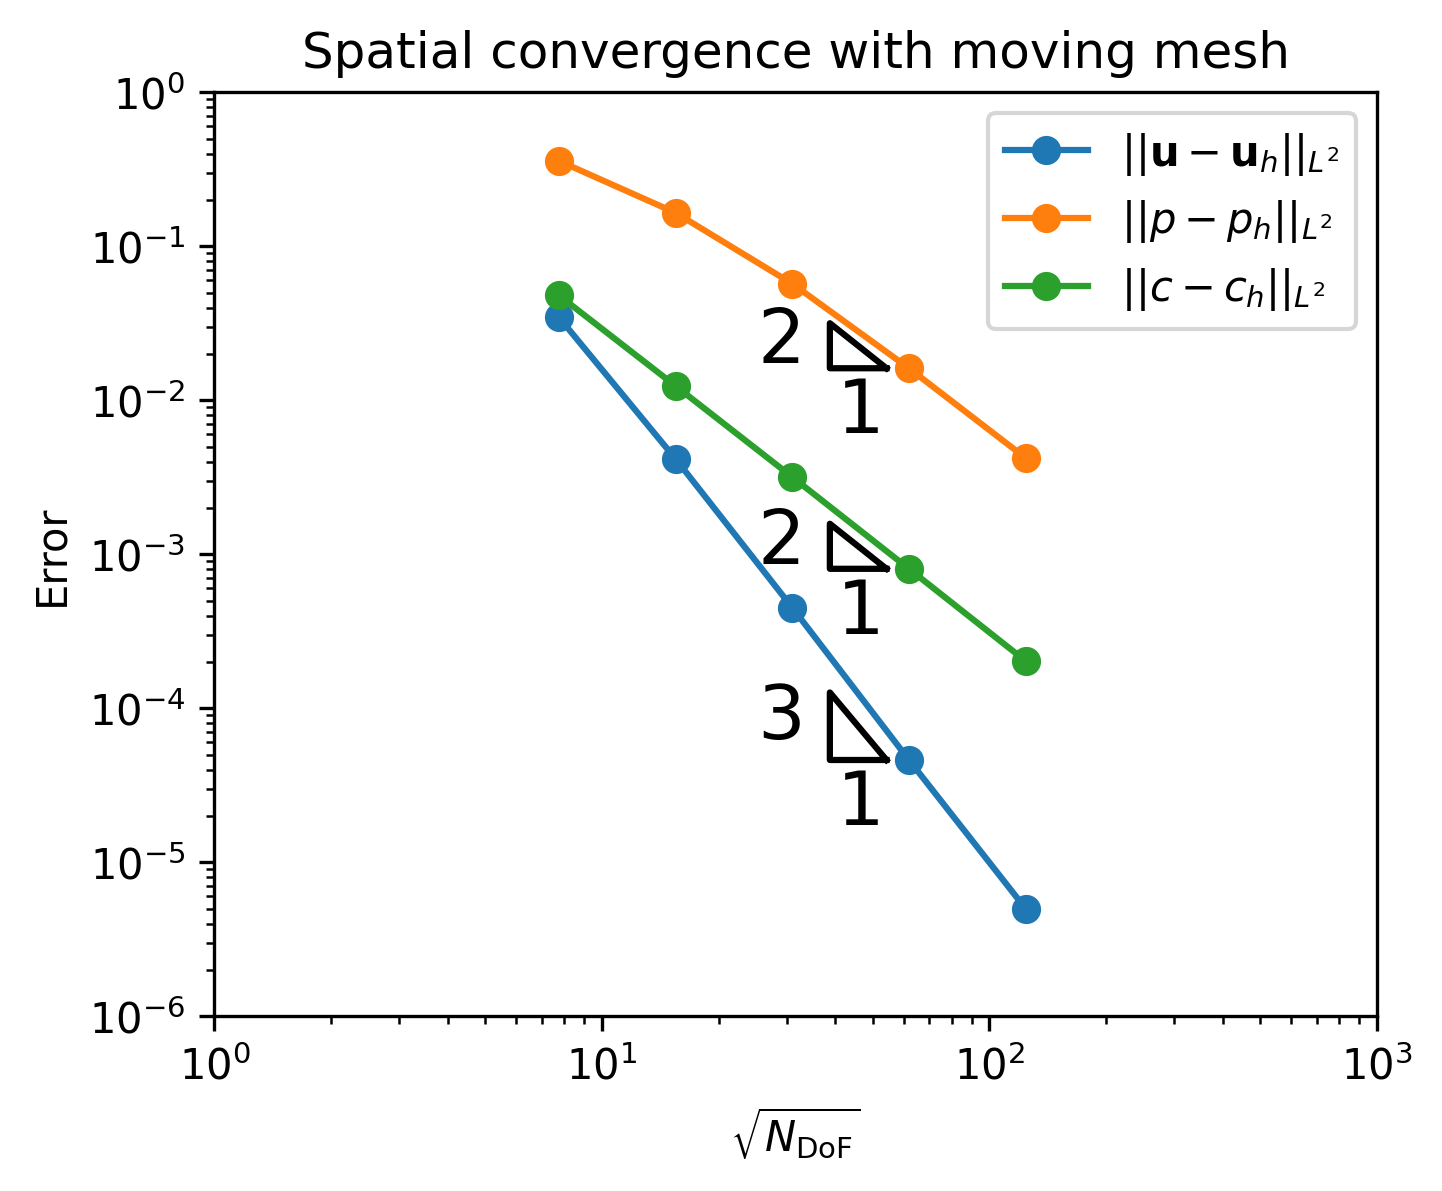
\includegraphics[width=\textwidth]{diagrams/results-convergence/mm_spatial_convergence.png}
                    \caption{}
                    \label{fig:mms-mm-convergence:space}
                \end{subfigure}
                \hfill
                \begin{subfigure}{0.45\textwidth}
                    \centering
                    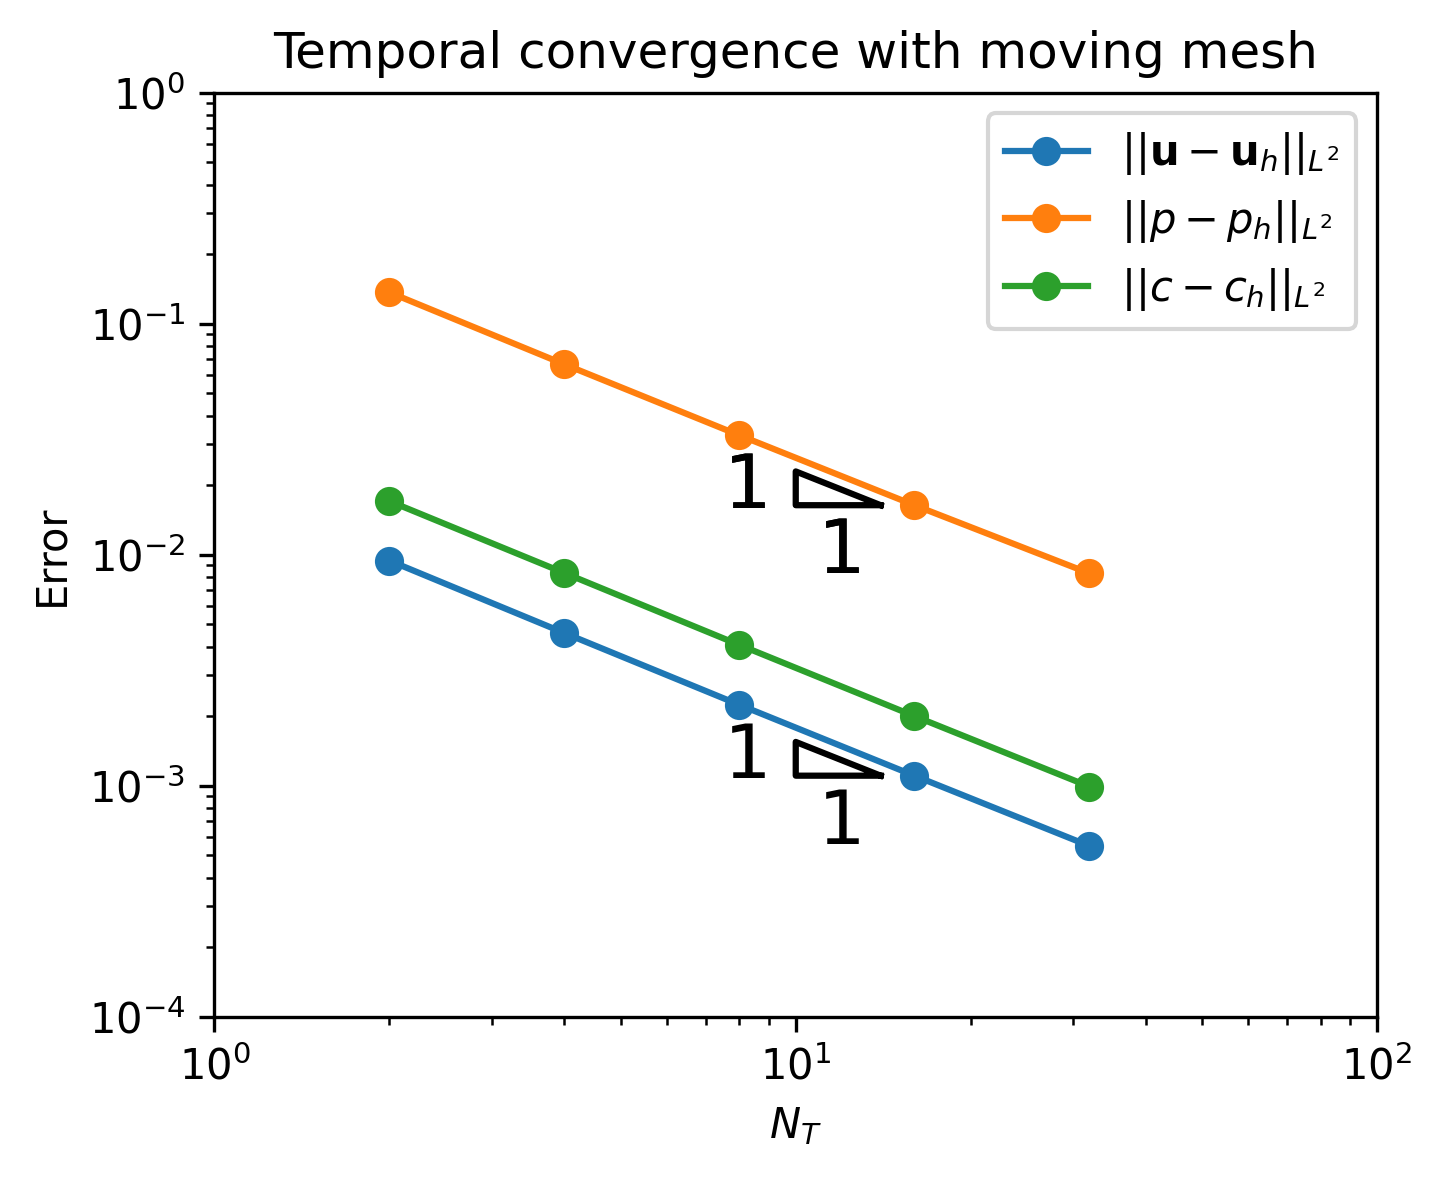
\includegraphics[width=\textwidth]{diagrams/results-convergence/mm_temporal_convergence.png}
                    \caption{}
                    \label{fig:mms-mm-convergence:time}
                \end{subfigure}
                \caption{Visualisations of the convergence rates of the tests outlined in \S\ref{sec:contractions:numerical-experiments:convergence}. Graphs show (a) spatial convergence, and (b) temporal convergence of the velocity, pressure, and oxygen concentration fields under a moving mesh.}
                \label{fig:mms-mm-convergence}
            \end{figure}

        \subsection{Boundary motion} \label{sec:contractions:numerical-experiments:boundary-movement}
            We now present an example of flow where part of the moving boundary has a no-slip boundary condition applied, which therefore influences flow dynamics. The flow problem we solve is again the Navier-Stokes-Darcy equations of Equation \eqref{eq:nsb}, initially on the unit square domain $\Omega^0 = [0, 1]^2$, where we for simplicity set $\mu = \rho = k = 1$, and set the smooth transition function $\Psi \equiv 1$ everywhere. Differing from the previous moving mesh numerical experiments, we apply a no-slip Dirichlet condition on the left and right sides of the domain, which for this moving domain problem is written $\vec{g}_D = \vec{w}$; we retain a free-flow Neumann condition of $\vec{g}_N = \vec{0}$ on the top and bottom of the domain. This choice of boundary conditions on the initial domain is visualised in Figures \ref{fig:square-solid-wall:0}.

            \begin{figure}
                \centering
                \begin{subfigure}{0.4\textwidth}
                    \centering
                    

\tikzset{every picture/.style={line width=0.75pt}} %set default line width to 0.75pt        
\resizebox{\textwidth}{!}{%
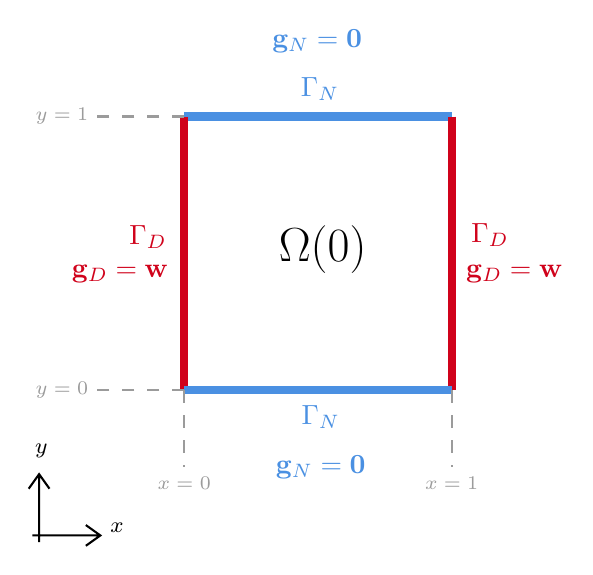
\begin{tikzpicture}[x=0.75pt,y=0.75pt,yscale=-1,xscale=1]
%uncomment if require: \path (0,336); %set diagram left start at 0, and has height of 336

%Straight Lines [id:da3775330886942099] 
\draw [color={rgb, 255:red, 74; green, 144; blue, 226 }  ,draw opacity=1 ][line width=3]    (113.28,81.05) -- (242.14,81.05) ;
%Straight Lines [id:da7311947956092497] 
\draw [color={rgb, 255:red, 208; green, 2; blue, 27 }  ,draw opacity=1 ][line width=3]    (242.14,81.05) -- (242.14,212.95) ;
%Straight Lines [id:da6649609020271117] 
\draw [color={rgb, 255:red, 208; green, 2; blue, 27 }  ,draw opacity=1 ][line width=3]    (113.28,81.05) -- (113.28,212.95) ;
%Straight Lines [id:da0032656115651366058] 
\draw [color={rgb, 255:red, 74; green, 144; blue, 226 }  ,draw opacity=1 ][line width=3]    (242.14,212.95) -- (113.28,212.95) ;
%Shape: Axis 2D [id:dp28368375799841394] 
\draw  (40.08,282.88) -- (72.88,282.88)(43.36,253.36) -- (43.36,286.16) (65.88,277.88) -- (72.88,282.88) -- (65.88,287.88) (38.36,260.36) -- (43.36,253.36) -- (48.36,260.36)  ;

%Straight Lines [id:da4221223762377593] 
\draw [color={rgb, 255:red, 155; green, 155; blue, 155 }  ,draw opacity=1 ] [dash pattern={on 4.5pt off 4.5pt}]  (113.28,212.95) -- (113.28,250) ;
%Straight Lines [id:da5345451203989031] 
\draw [color={rgb, 255:red, 155; green, 155; blue, 155 }  ,draw opacity=1 ] [dash pattern={on 4.5pt off 4.5pt}]  (242.14,212.95) -- (242.14,250) ;
%Straight Lines [id:da5891570191879292] 
\draw [color={rgb, 255:red, 155; green, 155; blue, 155 }  ,draw opacity=1 ] [dash pattern={on 4.5pt off 4.5pt}]  (113.28,212.95) -- (70.5,212.95) ;
%Straight Lines [id:da22019042876536155] 
\draw [color={rgb, 255:red, 155; green, 155; blue, 155 }  ,draw opacity=1 ] [dash pattern={on 4.5pt off 4.5pt}]  (113.28,81.05) -- (70.5,81.05) ;

% Text Node
\draw (106.32,138.93) node [anchor=east] [inner sep=0.75pt]  [color={rgb, 255:red, 208; green, 2; blue, 27 }  ,opacity=1 ]  {$\Gamma _{D}$};
% Text Node
\draw (250.14,138.04) node [anchor=west] [inner sep=0.75pt]  [color={rgb, 255:red, 208; green, 2; blue, 27 }  ,opacity=1 ]  {$\Gamma _{D}$};
% Text Node
\draw (178.66,74.95) node [anchor=south] [inner sep=0.75pt]  [color={rgb, 255:red, 74; green, 144; blue, 226 }  ,opacity=1 ]  {$\Gamma _{N}$};
% Text Node
\draw (179.09,218.96) node [anchor=north] [inner sep=0.75pt]  [color={rgb, 255:red, 74; green, 144; blue, 226 }  ,opacity=1 ]  {$\Gamma _{N}$};
% Text Node
\draw (107.05,150.96) node [anchor=north east] [inner sep=0.75pt]  [color={rgb, 255:red, 208; green, 2; blue, 27 }  ,opacity=1 ]  {$\mathbf{g}_{D} =\mathbf{w}$};
% Text Node
\draw (247.65,150.96) node [anchor=north west][inner sep=0.75pt]  [color={rgb, 255:red, 208; green, 2; blue, 27 }  ,opacity=1 ]  {$\mathbf{g}_{D} =\mathbf{w}$};
% Text Node
\draw (179.08,242.86) node [anchor=north] [inner sep=0.75pt]  [color={rgb, 255:red, 74; green, 144; blue, 226 }  ,opacity=1 ]  {$\mathbf{g}_{N} =\mathbf{0}$};
% Text Node
\draw (177.35,51.93) node [anchor=south] [inner sep=0.75pt]  [color={rgb, 255:red, 74; green, 144; blue, 226 }  ,opacity=1 ]  {$\mathbf{g}_{N} =\mathbf{0}$};
% Text Node
\draw (179.99,145.37) node  [font=\LARGE]  {$\Omega ( 0)$};
% Text Node
\draw (76.26,279.4) node [anchor=west] [inner sep=0.75pt]  [font=\footnotesize]  {$x$};
% Text Node
\draw (44.4,246.95) node [anchor=south] [inner sep=0.75pt]  [font=\footnotesize]  {$y$};
% Text Node
\draw (113.28,253.4) node [anchor=north] [inner sep=0.75pt]  [font=\scriptsize,color={rgb, 255:red, 155; green, 155; blue, 155 }  ,opacity=1 ]  {$x=0$};
% Text Node
\draw (242.14,253.4) node [anchor=north] [inner sep=0.75pt]  [font=\scriptsize,color={rgb, 255:red, 155; green, 155; blue, 155 }  ,opacity=1 ]  {$x=1$};
% Text Node
\draw (68.5,212.95) node [anchor=east] [inner sep=0.75pt]  [font=\scriptsize,color={rgb, 255:red, 155; green, 155; blue, 155 }  ,opacity=1 ]  {$y=0$};
% Text Node
\draw (68.5,81.05) node [anchor=east] [inner sep=0.75pt]  [font=\scriptsize,color={rgb, 255:red, 155; green, 155; blue, 155 }  ,opacity=1 ]  {$y=1$};


\end{tikzpicture}
}
                    \caption{}
                    \label{fig:square-solid-wall:0}
                \end{subfigure}
                \hfill
                \begin{subfigure}{0.53\textwidth}
                    \centering
                    

\tikzset{every picture/.style={line width=0.75pt}} %set default line width to 0.75pt        
\resizebox{\textwidth}{!}{%
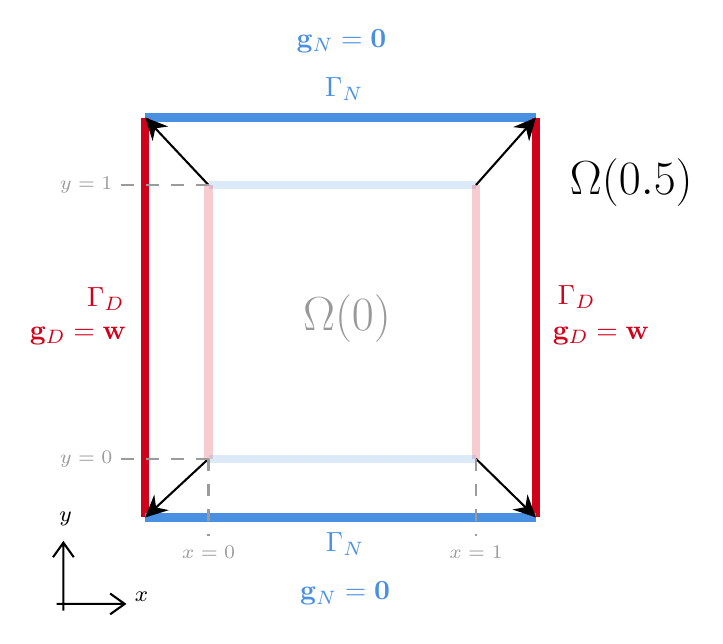
\begin{tikzpicture}[x=0.75pt,y=0.75pt,yscale=-1,xscale=1]
%uncomment if require: \path (0,350); %set diagram left start at 0, and has height of 350

%Straight Lines [id:da3911785235524641] 
\draw [color={rgb, 255:red, 74; green, 144; blue, 226 }  ,draw opacity=1 ][line width=3]    (98.78,72.15) -- (287,72.15) ;
%Straight Lines [id:da08153744945246588] 
\draw [color={rgb, 255:red, 208; green, 2; blue, 27 }  ,draw opacity=1 ][line width=3]    (287,72.15) -- (287,264.82) ;
%Straight Lines [id:da5688674307213424] 
\draw [color={rgb, 255:red, 208; green, 2; blue, 27 }  ,draw opacity=1 ][line width=3]    (98.78,72.15) -- (98.78,264.82) ;
%Straight Lines [id:da13408740199002578] 
\draw [color={rgb, 255:red, 74; green, 144; blue, 226 }  ,draw opacity=1 ][line width=3]    (287,264.82) -- (98.78,264.82) ;
%Straight Lines [id:da8870048899559595] 
\draw [color={rgb, 255:red, 74; green, 144; blue, 226 }  ,draw opacity=0.2 ][line width=3]    (129.28,104.65) -- (258.14,104.65) ;
%Straight Lines [id:da8723650118672401] 
\draw [color={rgb, 255:red, 208; green, 2; blue, 27 }  ,draw opacity=0.2 ][line width=3]    (258.14,104.65) -- (258.14,236.55) ;
%Straight Lines [id:da4357741269330557] 
\draw [color={rgb, 255:red, 208; green, 2; blue, 27 }  ,draw opacity=0.2 ][line width=3]    (129.28,104.65) -- (129.28,236.55) ;
%Straight Lines [id:da9191492030234965] 
\draw [color={rgb, 255:red, 74; green, 144; blue, 226 }  ,draw opacity=0.2 ][line width=3]    (258.14,236.55) -- (129.28,236.55) ;
%Shape: Axis 2D [id:dp9350720821526224] 
\draw  (56.08,306.48) -- (88.88,306.48)(59.36,276.96) -- (59.36,309.76) (81.88,301.48) -- (88.88,306.48) -- (81.88,311.48) (54.36,283.96) -- (59.36,276.96) -- (64.36,283.96)  ;

%Straight Lines [id:da021521710554898155] 
\draw    (129.28,104.65) -- (100.83,74.34) ;
\draw [shift={(98.78,72.15)}, rotate = 46.82] [fill={rgb, 255:red, 0; green, 0; blue, 0 }  ][line width=0.08]  [draw opacity=0] (10.72,-5.15) -- (0,0) -- (10.72,5.15) -- (7.12,0) -- cycle    ;
%Straight Lines [id:da8341315604563517] 
\draw    (258.14,104.65) -- (285.01,74.39) ;
\draw [shift={(287,72.15)}, rotate = 131.61] [fill={rgb, 255:red, 0; green, 0; blue, 0 }  ][line width=0.08]  [draw opacity=0] (10.72,-5.15) -- (0,0) -- (10.72,5.15) -- (7.12,0) -- cycle    ;
%Straight Lines [id:da6015135889734096] 
\draw    (258.14,236.55) -- (284.86,262.72) ;
\draw [shift={(287,264.82)}, rotate = 224.4] [fill={rgb, 255:red, 0; green, 0; blue, 0 }  ][line width=0.08]  [draw opacity=0] (10.72,-5.15) -- (0,0) -- (10.72,5.15) -- (7.12,0) -- cycle    ;
%Straight Lines [id:da44271674446744247] 
\draw    (129.28,236.55) -- (100.98,262.78) ;
\draw [shift={(98.78,264.82)}, rotate = 317.18] [fill={rgb, 255:red, 0; green, 0; blue, 0 }  ][line width=0.08]  [draw opacity=0] (10.72,-5.15) -- (0,0) -- (10.72,5.15) -- (7.12,0) -- cycle    ;
%Straight Lines [id:da8787304201926478] 
\draw [color={rgb, 255:red, 155; green, 155; blue, 155 }  ,draw opacity=1 ] [dash pattern={on 4.5pt off 4.5pt}]  (129.28,236.55) -- (129.28,273.6) ;
%Straight Lines [id:da19489772630369218] 
\draw [color={rgb, 255:red, 155; green, 155; blue, 155 }  ,draw opacity=1 ] [dash pattern={on 4.5pt off 4.5pt}]  (258.14,236.55) -- (258.14,273.6) ;
%Straight Lines [id:da9299742276817373] 
\draw [color={rgb, 255:red, 155; green, 155; blue, 155 }  ,draw opacity=1 ] [dash pattern={on 4.5pt off 4.5pt}]  (129.28,236.55) -- (86.5,236.55) ;
%Straight Lines [id:da941430709775763] 
\draw [color={rgb, 255:red, 155; green, 155; blue, 155 }  ,draw opacity=1 ] [dash pattern={on 4.5pt off 4.5pt}]  (129.28,104.65) -- (86.5,104.65) ;

% Text Node
\draw (90.32,159.53) node [anchor=east] [inner sep=0.75pt]  [color={rgb, 255:red, 208; green, 2; blue, 27 }  ,opacity=1 ]  {$\Gamma _{D}$};
% Text Node
\draw (296.14,158.64) node [anchor=west] [inner sep=0.75pt]  [color={rgb, 255:red, 208; green, 2; blue, 27 }  ,opacity=1 ]  {$\Gamma _{D}$};
% Text Node
\draw (194.66,65.55) node [anchor=south] [inner sep=0.75pt]  [color={rgb, 255:red, 74; green, 144; blue, 226 }  ,opacity=1 ]  {$\Gamma _{N}$};
% Text Node
\draw (195.09,270.56) node [anchor=north] [inner sep=0.75pt]  [color={rgb, 255:red, 74; green, 144; blue, 226 }  ,opacity=1 ]  {$\Gamma _{N}$};
% Text Node
\draw (91.05,171.56) node [anchor=north east] [inner sep=0.75pt]  [color={rgb, 255:red, 208; green, 2; blue, 27 }  ,opacity=1 ]  {$\mathbf{g}_{D} =\mathbf{w}$};
% Text Node
\draw (293.65,171.56) node [anchor=north west][inner sep=0.75pt]  [color={rgb, 255:red, 208; green, 2; blue, 27 }  ,opacity=1 ]  {$\mathbf{g}_{D} =\mathbf{w}$};
% Text Node
\draw (195.08,294.46) node [anchor=north] [inner sep=0.75pt]  [color={rgb, 255:red, 74; green, 144; blue, 226 }  ,opacity=1 ]  {$\mathbf{g}_{N} =\mathbf{0}$};
% Text Node
\draw (193.35,42.53) node [anchor=south] [inner sep=0.75pt]  [color={rgb, 255:red, 74; green, 144; blue, 226 }  ,opacity=1 ]  {$\mathbf{g}_{N} =\mathbf{0}$};
% Text Node
\draw (195.99,168.97) node  [font=\LARGE,color={rgb, 255:red, 0; green, 0; blue, 0 }  ,opacity=0.4 ]  {$\Omega ( 0)$};
% Text Node
\draw (301.93,103.47) node [anchor=west] [inner sep=0.75pt]  [font=\LARGE,color={rgb, 255:red, 0; green, 0; blue, 0 }  ,opacity=1 ]  {$\Omega ( 0.5)$};
% Text Node
\draw (129.28,277) node [anchor=north] [inner sep=0.75pt]  [font=\scriptsize,color={rgb, 255:red, 155; green, 155; blue, 155 }  ,opacity=1 ]  {$x=0$};
% Text Node
\draw (258.14,277) node [anchor=north] [inner sep=0.75pt]  [font=\scriptsize,color={rgb, 255:red, 155; green, 155; blue, 155 }  ,opacity=1 ]  {$x=1$};
% Text Node
\draw (84.5,236.55) node [anchor=east] [inner sep=0.75pt]  [font=\scriptsize,color={rgb, 255:red, 155; green, 155; blue, 155 }  ,opacity=1 ]  {$y=0$};
% Text Node
\draw (84.5,104.65) node [anchor=east] [inner sep=0.75pt]  [font=\scriptsize,color={rgb, 255:red, 155; green, 155; blue, 155 }  ,opacity=1 ]  {$y=1$};
% Text Node
\draw (92.26,303) node [anchor=west] [inner sep=0.75pt]  [font=\footnotesize]  {$x$};
% Text Node
\draw (60.4,270.55) node [anchor=south] [inner sep=0.75pt]  [font=\footnotesize]  {$y$};


\end{tikzpicture}
}
                    \caption{}
                    \label{fig:square-solid-wall:later}
                \end{subfigure}
                \caption{Visualisation of the boundary conditions applied to the problem described in \S\ref{sec:contractions:numerical-experiments:boundary-movement}, which applies a zero Neumann condition on the top and bottom sides of the domain, and a no-slip Dirichlet condition on the left and right sides. $\Omega$ is shown at times (a) $t=0$, and (b) $t=0.5$ for the domain velocity detailed in Equation \eqref{eq:oscillating-mesh-velocity} and \S\ref{sec:contractions:numerical-experiments:boundary-movement}.}
                \label{fig:square-solid-wall}
            \end{figure}
            
            We begin the simulation with an initial condition of $\vec{u}_h^0 \equiv \vec{0}$ and run between times $t \in [0, 1]$, with time-step size $\Delta t = 0.01$. We select the domain velocity $\vec{w} \equiv (w_1, w_2)^\intercal$ as
            \begin{subequations}
                \begin{equation}
                    w_1 = W (x - x_c) \sin\left(\frac{2 \pi t - T_0}{T}\right),
                    \label{eq:oscillating-mesh-velocity:1}
                \end{equation}
                \begin{equation}
                    w_2 = W (y - y_c) \sin\left(\frac{2 \pi t - T_0}{T}\right),
                    \label{eq:oscillating-mesh-velocity:2}
                \end{equation}%
                \label{eq:oscillating-mesh-velocity}%
            \end{subequations}%
            where we select $x_c = y_c = 0.5$, $T_0 = 0$, $T = 1$, and $W = 1$ here. This domain velocity corresponds to smooth expansion and contraction about centre $(x_c, y_c) = (0.5, 0.5)$ for $t \in [0, 1]$, with a minimal domain area of $\Omega$ at $t = 0$ and $t=1$, and a maximal area at $t = 0.5$. Furthermore, we note that this gives a maximal rate of expansion at $t = 0.25$ and maximal rate of deflation at $t = 0.75$. The maximum domain size at $t=0.5$ is visualised in Figure \ref{fig:square-solid-wall:later}.
            
            Figures \ref{fig:square-solid-wall-flow:02}--\ref{fig:square-solid-wall-flow:75} respectively visualise the flow at times $t=0.02$, $t=0.25$, $t=0.52$, and $t=0.75$. A video visualising the velocity field through time at every time-step is available here\footnote{\url{https://r.blakey.family/phd-video-mmv-square}}. At $t = 0.02$, Figure \ref{fig:square-solid-wall-flow:02} shows the flow drawn through the top and bottom sides and aligning in the direction of the domain velocity on the boundary, which is at that moment pointing outward from the centre of the square domain. The domain velocity then accelerates up to a maximum domain velocity at $t = 0.25$, as illustrated in Figure \ref{fig:square-solid-wall-flow:25}, which shows high-speed blood concentrated in the centre of the top and bottom sides, and also in the four corners of the domain. The domain velocity then decelerates as the area reaches its maximum size at $t=0.5$; Figure \ref{fig:square-solid-wall-flow:52} shows the velocity field at $t = 0.52$, just after the maximum area is reached, where we note the reversal in the streamline directions as the domain begins to contract and eject flow out of the top and bottom sides. Finally, Figure \ref{fig:square-solid-wall-flow:75} shows the domain at $t = 0.75$ at the most rapid point of contraction, which unsurprisingly looks very similar to the flow at $t=0.25$ except for a reversal in flow direction.
            
            \begin{figure}
                \begin{centering}
                    %%%%%
                    \begin{subfigure}{0.45\textwidth}
                        \begin{centering}
                            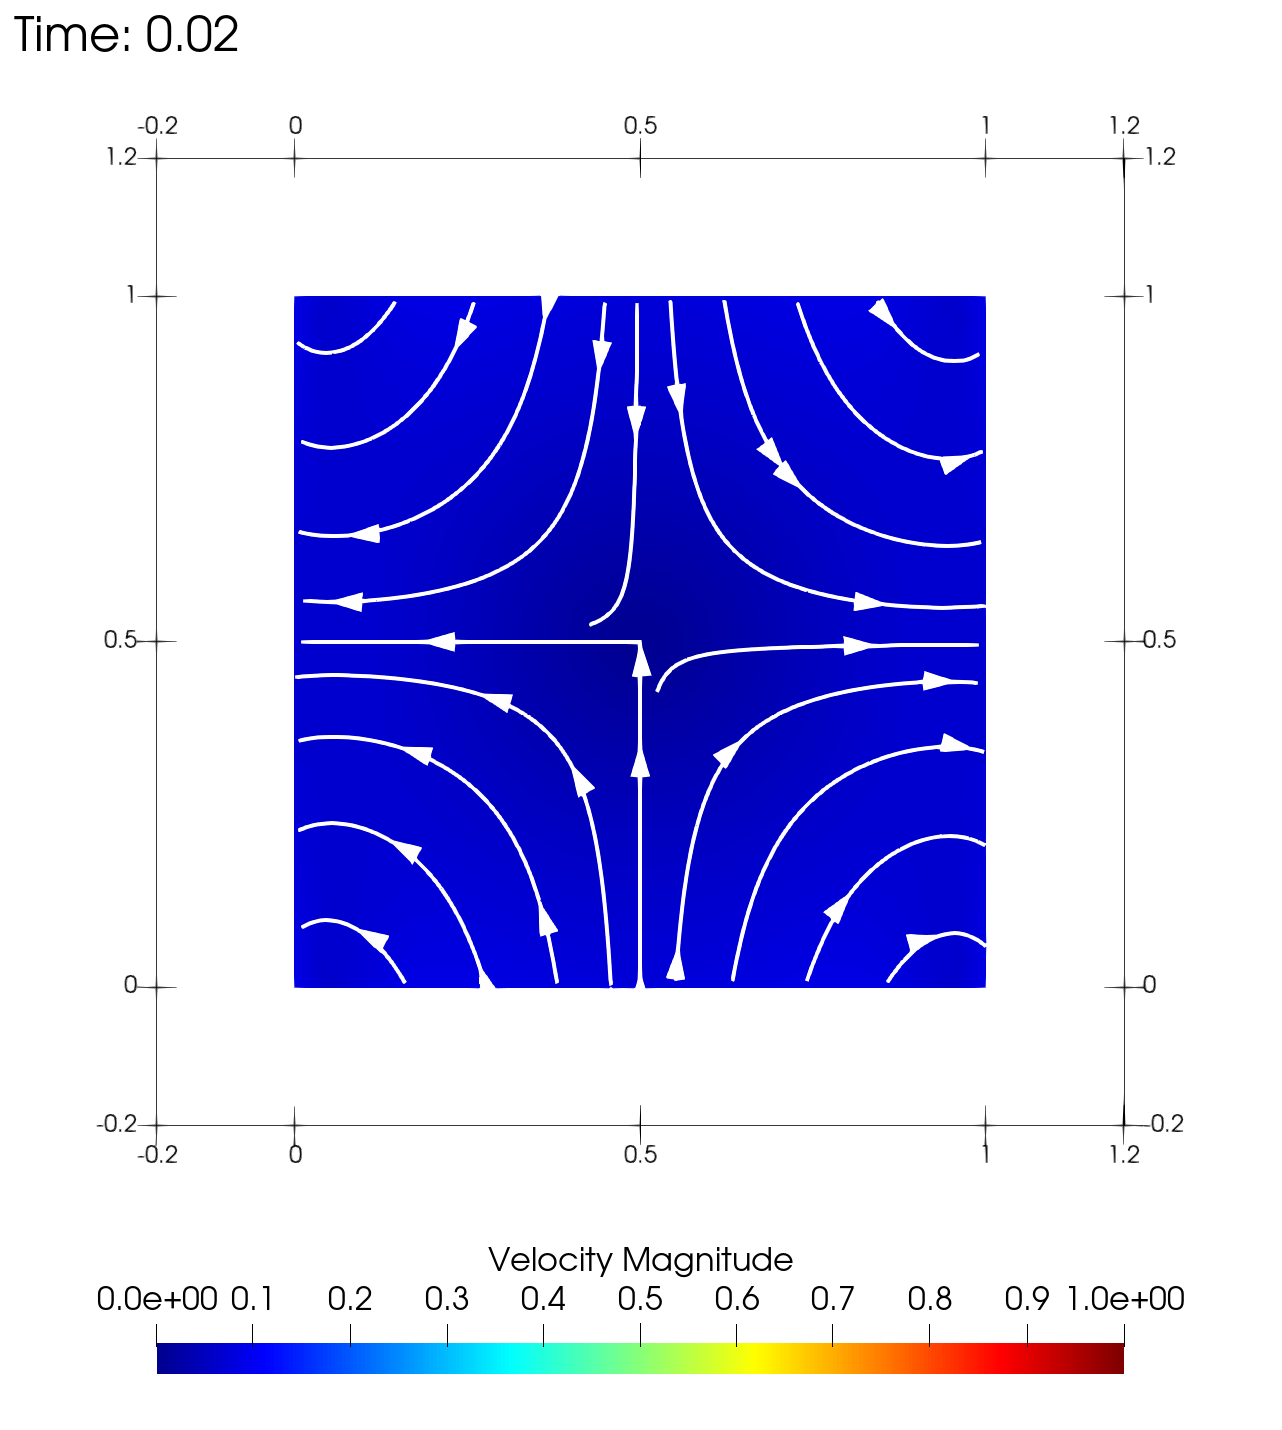
\includegraphics[width=\textwidth]{diagrams/results-contractions/mm_5_white.0002.png}
                            \caption{}
                            \label{fig:square-solid-wall-flow:02}
                        \end{centering}
                    \end{subfigure}
                    \begin{subfigure}{0.45\textwidth}
                        \begin{centering}
                            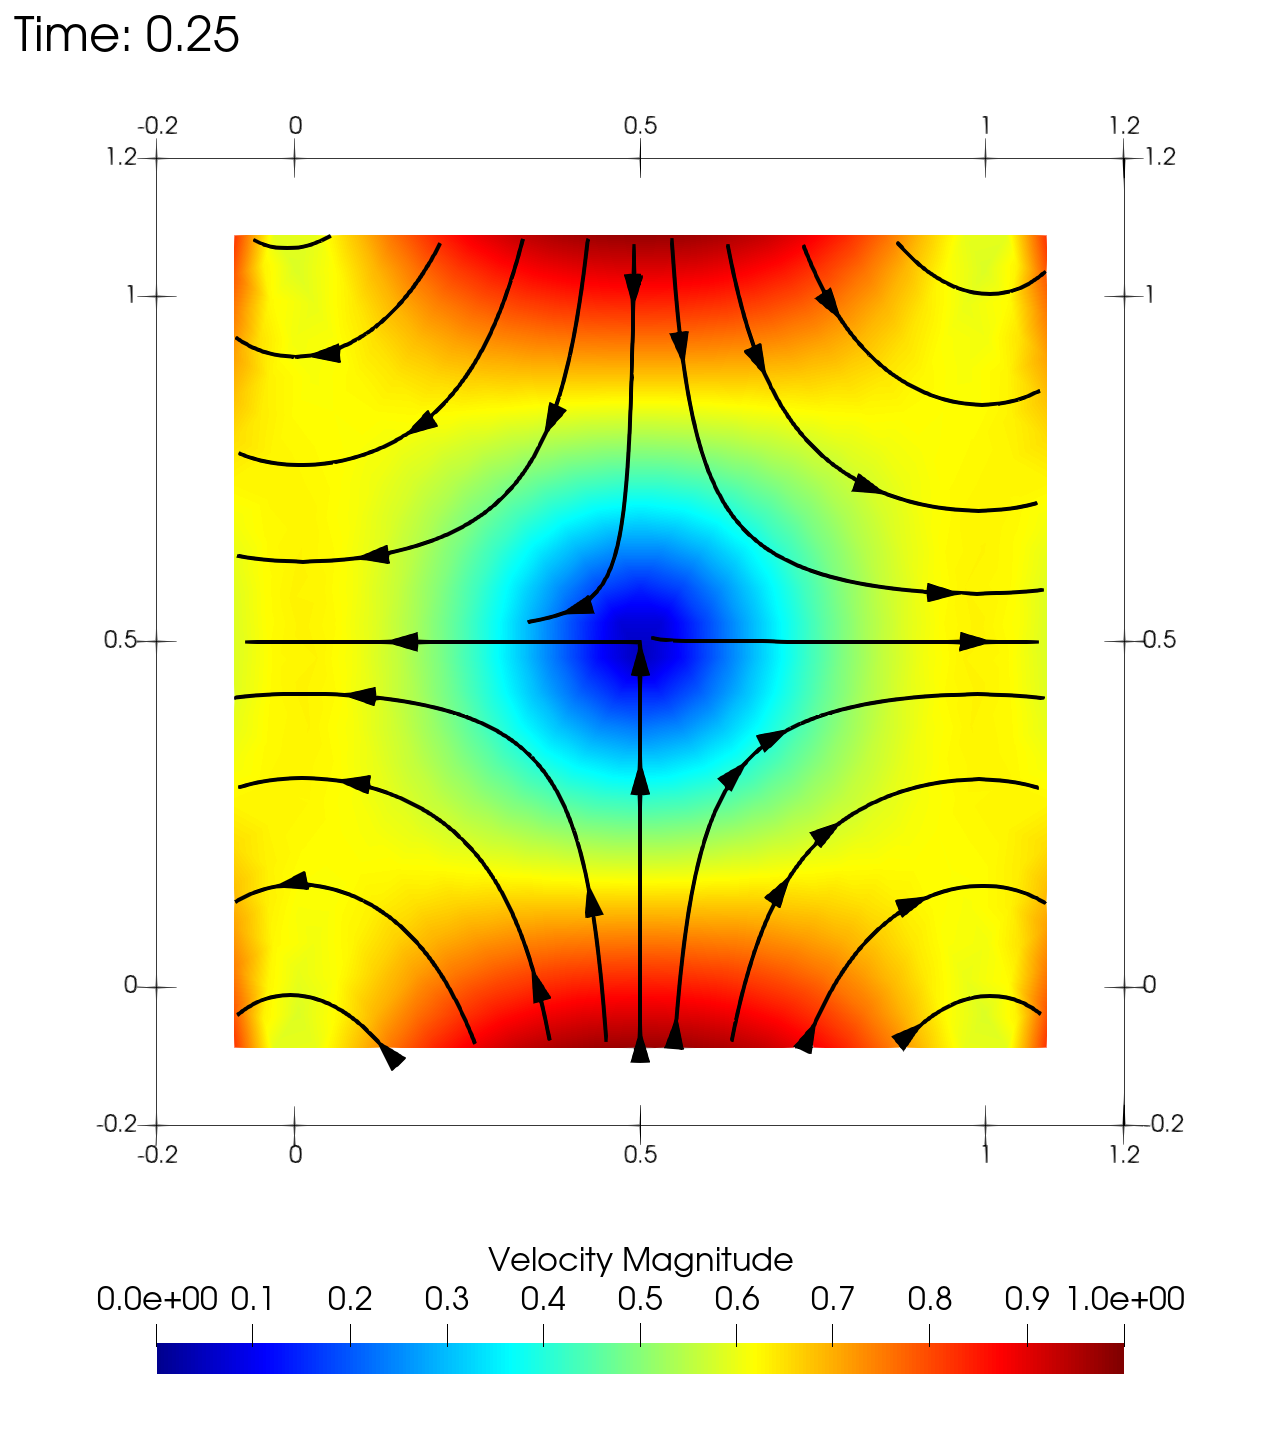
\includegraphics[width=\textwidth]{diagrams/results-contractions/mm_5_black.0025.png}
                            \caption{}
                            \label{fig:square-solid-wall-flow:25}
                        \end{centering}
                    \end{subfigure}
                    \begin{subfigure}{0.45\textwidth}
                        \begin{centering}
                            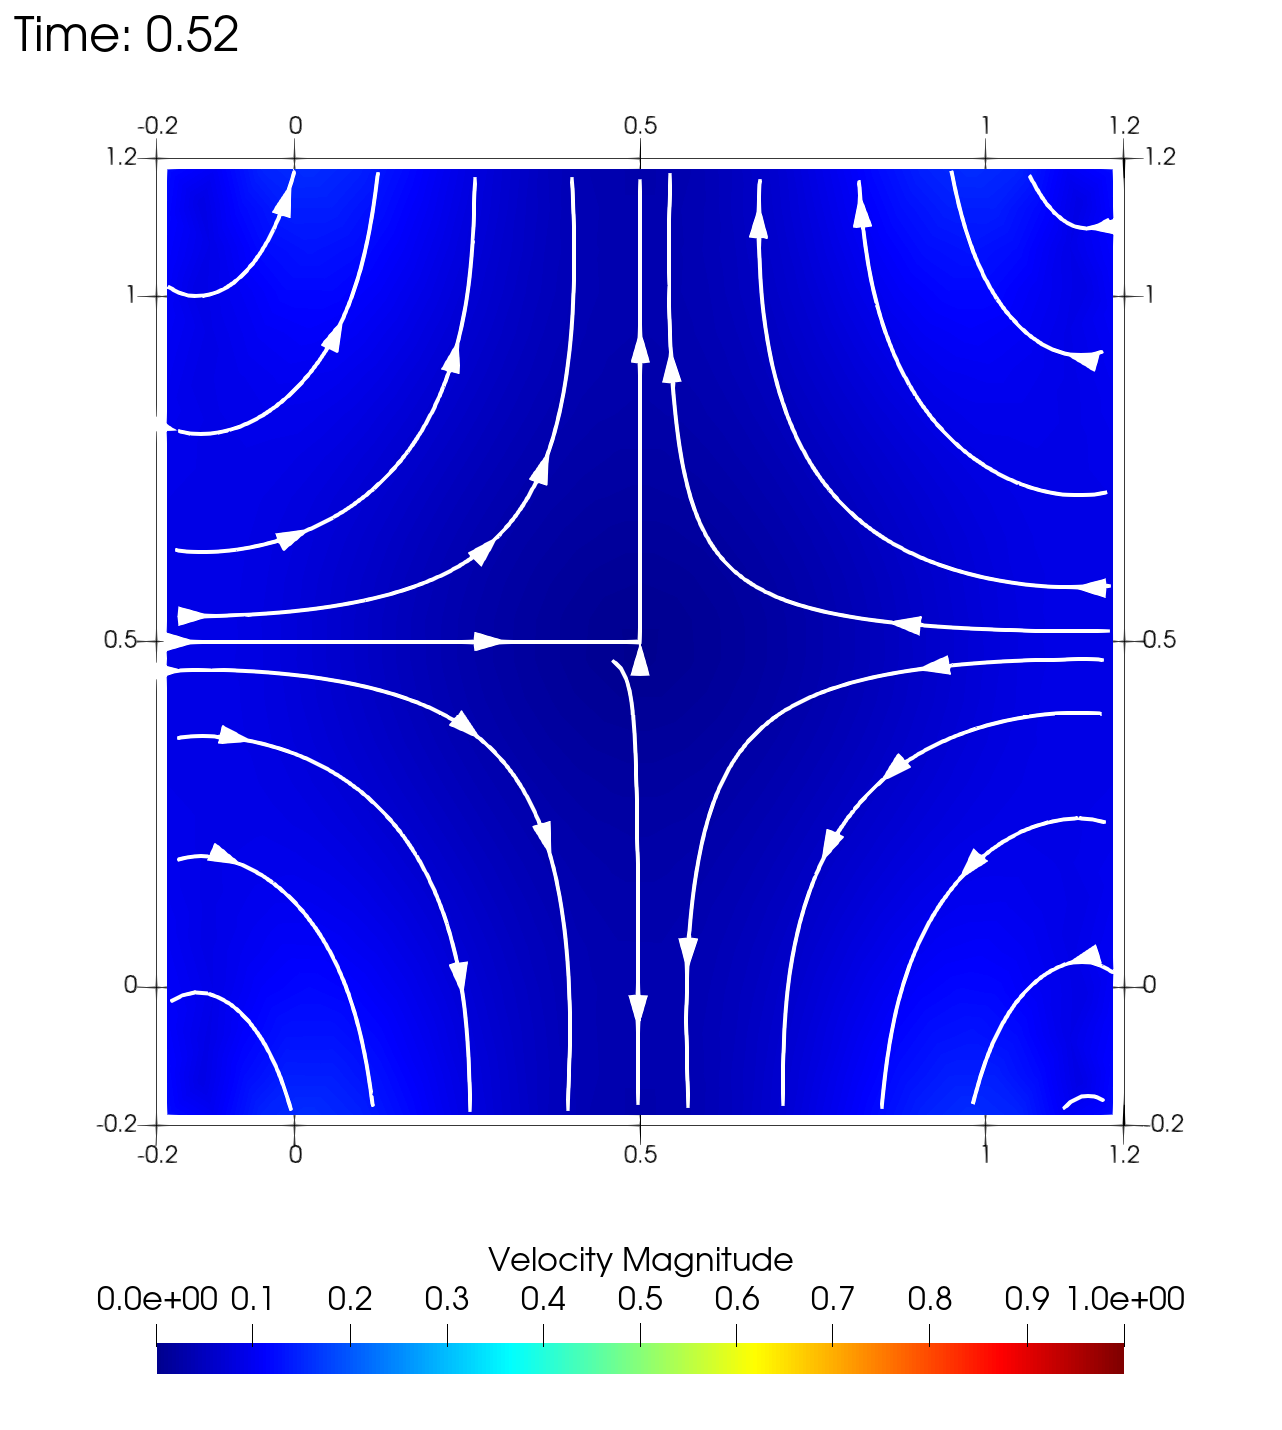
\includegraphics[width=\textwidth]{diagrams/results-contractions/mm_5_white.0052.png}
                            \caption{}
                            \label{fig:square-solid-wall-flow:52}
                        \end{centering}
                    \end{subfigure}
                    \begin{subfigure}{0.45\textwidth}
                        \begin{centering}
                            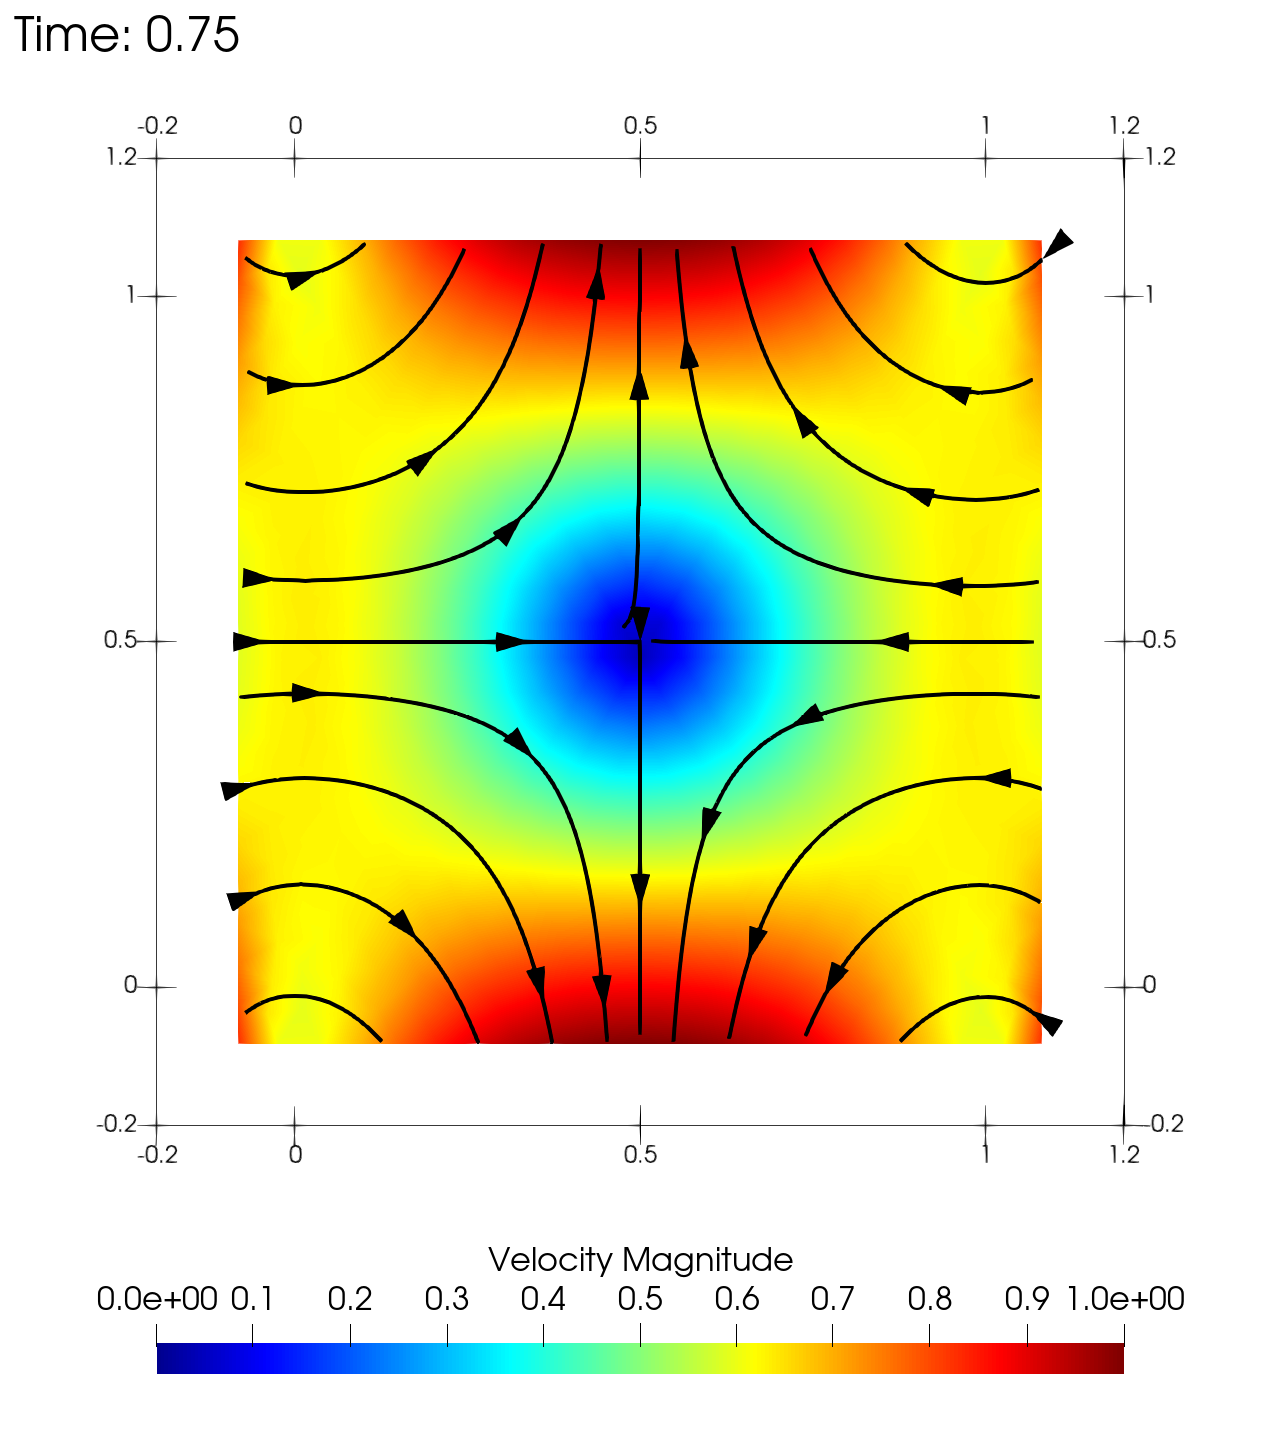
\includegraphics[width=\textwidth]{diagrams/results-contractions/mm_5_black.0075.png}
                            \caption{}
                            \label{fig:square-solid-wall-flow:75}
                        \end{centering}
                    \end{subfigure}
                \end{centering}
                \caption{Visualisations of flow for four instances in time for the problem in \S\ref{sec:contractions:numerical-experiments:boundary-movement}. (a)-(d) respectively show flow at $t=0.02$, $t=0.25$, $t=0.52$, $t=0.75$. Linear colour scaling is shown for $|\vec{u}| \in [0, 1]$ with black or white streamlines shown on top. Axes are shown surrounding the domain, showing the domain of size $\Omega = [0, 1]^2$ at $t \approx 0$ and $\Omega \approx [-0.2, 1.2]^2$ at $t \approx 0.5$.}
                \label{fig:square-solid-wall-flow}
            \end{figure}

            In order to model flow in a contracting placenta, we will now apply the numerical methods from \S\ref{sec:contractions:dgfem-discretisation} to NSD with placental flow parameters and the asymmetric placenta problem from \S\ref{sec:numerical-methods:blood-flow-experiments:asymmetric}.

    \section{Preliminary utero-placental pump motion} \label{sec:contractions:placenta}
        The utero-placental pump (or placental contraction) is a newly discovered phenomenon, first reported by \citeauthor{dellschaftHaemodynamicsHumanPlacenta2020} \cite{dellschaftHaemodynamicsHumanPlacenta2020} in \citeyear{dellschaftHaemodynamicsHumanPlacenta2020}. This phenomenon is distinct from other types of contractions, as it involves contractions of the placenta, rather than contractions such as Braxton-Hicks contractions, which instead involve contractions of the entire uterus \cite{togashiSustainedUterineContractions1993}. \citeauthor{dellschaftHaemodynamicsHumanPlacenta2020} \cite{dellschaftHaemodynamicsHumanPlacenta2020} reported that the placenta was observed over $10$-minute intervals to periodically reduce by up to $40\%$ in volume, resulting in the periodic ejection of blood from the IVS. The mechanism of these contractions is not yet known, but it is thought that these contractions may be related to previous reports of contracting villous trees \cite{farleyContractilePropertiesHuman2004,dellschaftHaemodynamicsHumanPlacenta2020}. One theory of the evolutionary role of these contractions is that they assist maternal circulation by ejecting stagnant deoxygenated blood so that it may be replaced by freshly oxygenated blood; however, this is yet to be shown experimentally \cite{dellschaftHaemodynamicsHumanPlacenta2020}.

        In this section, we will prescribe a simple domain velocity that is inspired by MRI scan data. Using this domain velocity, we will then compute the resulting flow and oxygen concentration fields using the moving mesh discretisation presented in \S\ref{sec:contractions:dgfem-discretisation}.

        \subsection{Selection of domain velocity} \label{sec:contractions:placenta:mesh-velocity}
            We begin by using the data from \citeauthor{gowlandCharacterisingPlacentalContractions2024} \cite{gowlandCharacterisingPlacentalContractions2024}, which is reproduced in Figure \ref{fig:contraction-data:raw} and shows various quantities calculated from MRI scan data during a placental contraction. We choose to focus specifically on the volume change during the period of fastest volume reduction, which is indicated in the black box. The volume change data here is calculated by tracing the placenta outline of a 3D stack of 2D MRI scan images, and is measured against the initial placental volume calculated at time $t = 0$.

            \begin{figure}
                \centering
                \begin{subfigure}{\textwidth}
                    \centering
                    

\tikzset{every picture/.style={line width=0.75pt}} %set default line width to 0.75pt        

\begin{tikzpicture}[x=0.75pt,y=0.75pt,yscale=-1,xscale=1]
%uncomment if require: \path (0,300); %set diagram left start at 0, and has height of 300

%Image [id:dp23581150653458827] 
\draw (294.71,143) node  {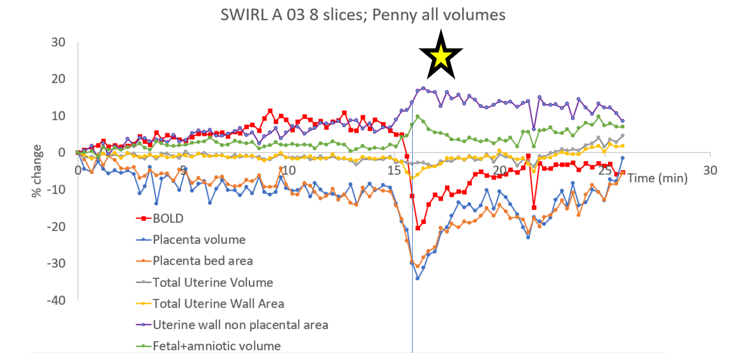
\includegraphics[width=415.07pt,height=198pt]{diagrams/other-paper-figures/gowland2024_contraction-data.png}};
%Shape: Rectangle [id:dp0616002982809305] 
\draw  [line width=3]  (285,107) -- (347,107) -- (347,230) -- (285,230) -- cycle ;
%Shape: Rectangle [id:dp37370129948188047] 
\draw  [draw opacity=0][fill={rgb, 255:red, 0; green, 0; blue, 0 }  ,fill opacity=0.2 ] (18,11) -- (108.67,11) -- (108.67,274) -- (18,274) -- cycle ;
%Shape: Rectangle [id:dp08993919230122849] 
\draw  [draw opacity=0][fill={rgb, 255:red, 0; green, 0; blue, 0 }  ,fill opacity=0.2 ] (347,11) -- (571,11) -- (571,274) -- (347,274) -- cycle ;
%Shape: Rectangle [id:dp06260699697048411] 
\draw  [draw opacity=0][fill={rgb, 255:red, 0; green, 0; blue, 0 }  ,fill opacity=0.2 ] (285.33,11) -- (347,11) -- (347,107) -- (285.33,107) -- cycle ;
%Shape: Rectangle [id:dp8344768536283782] 
\draw  [draw opacity=0][fill={rgb, 255:red, 0; green, 0; blue, 0 }  ,fill opacity=0.2 ] (285.33,230.33) -- (347,230.33) -- (347,274) -- (285.33,274) -- cycle ;
%Shape: Rectangle [id:dp7625893108020545] 
\draw  [line width=3]  (108.33,182.67) -- (208.67,182.67) -- (208.67,197.67) -- (108.33,197.67) -- cycle ;
%Shape: Rectangle [id:dp9788521517108135] 
\draw  [draw opacity=0][fill={rgb, 255:red, 0; green, 0; blue, 0 }  ,fill opacity=0.2 ] (208.67,11) -- (285.33,11) -- (285.33,274) -- (208.67,274) -- cycle ;
%Shape: Rectangle [id:dp9892312056868955] 
\draw  [draw opacity=0][fill={rgb, 255:red, 0; green, 0; blue, 0 }  ,fill opacity=0.2 ] (108.67,11) -- (208.67,11) -- (208.67,181) -- (108.67,181) -- cycle ;
%Shape: Rectangle [id:dp472204421176478] 
\draw  [draw opacity=0][fill={rgb, 255:red, 0; green, 0; blue, 0 }  ,fill opacity=0.2 ] (108.67,197.67) -- (208.67,197.67) -- (208.67,274) -- (108.67,274) -- cycle ;




\end{tikzpicture}

                    \caption{}
                    \label{fig:contraction-data:raw}
                \end{subfigure}
                \begin{subfigure}{\textwidth}
                    \centering
                    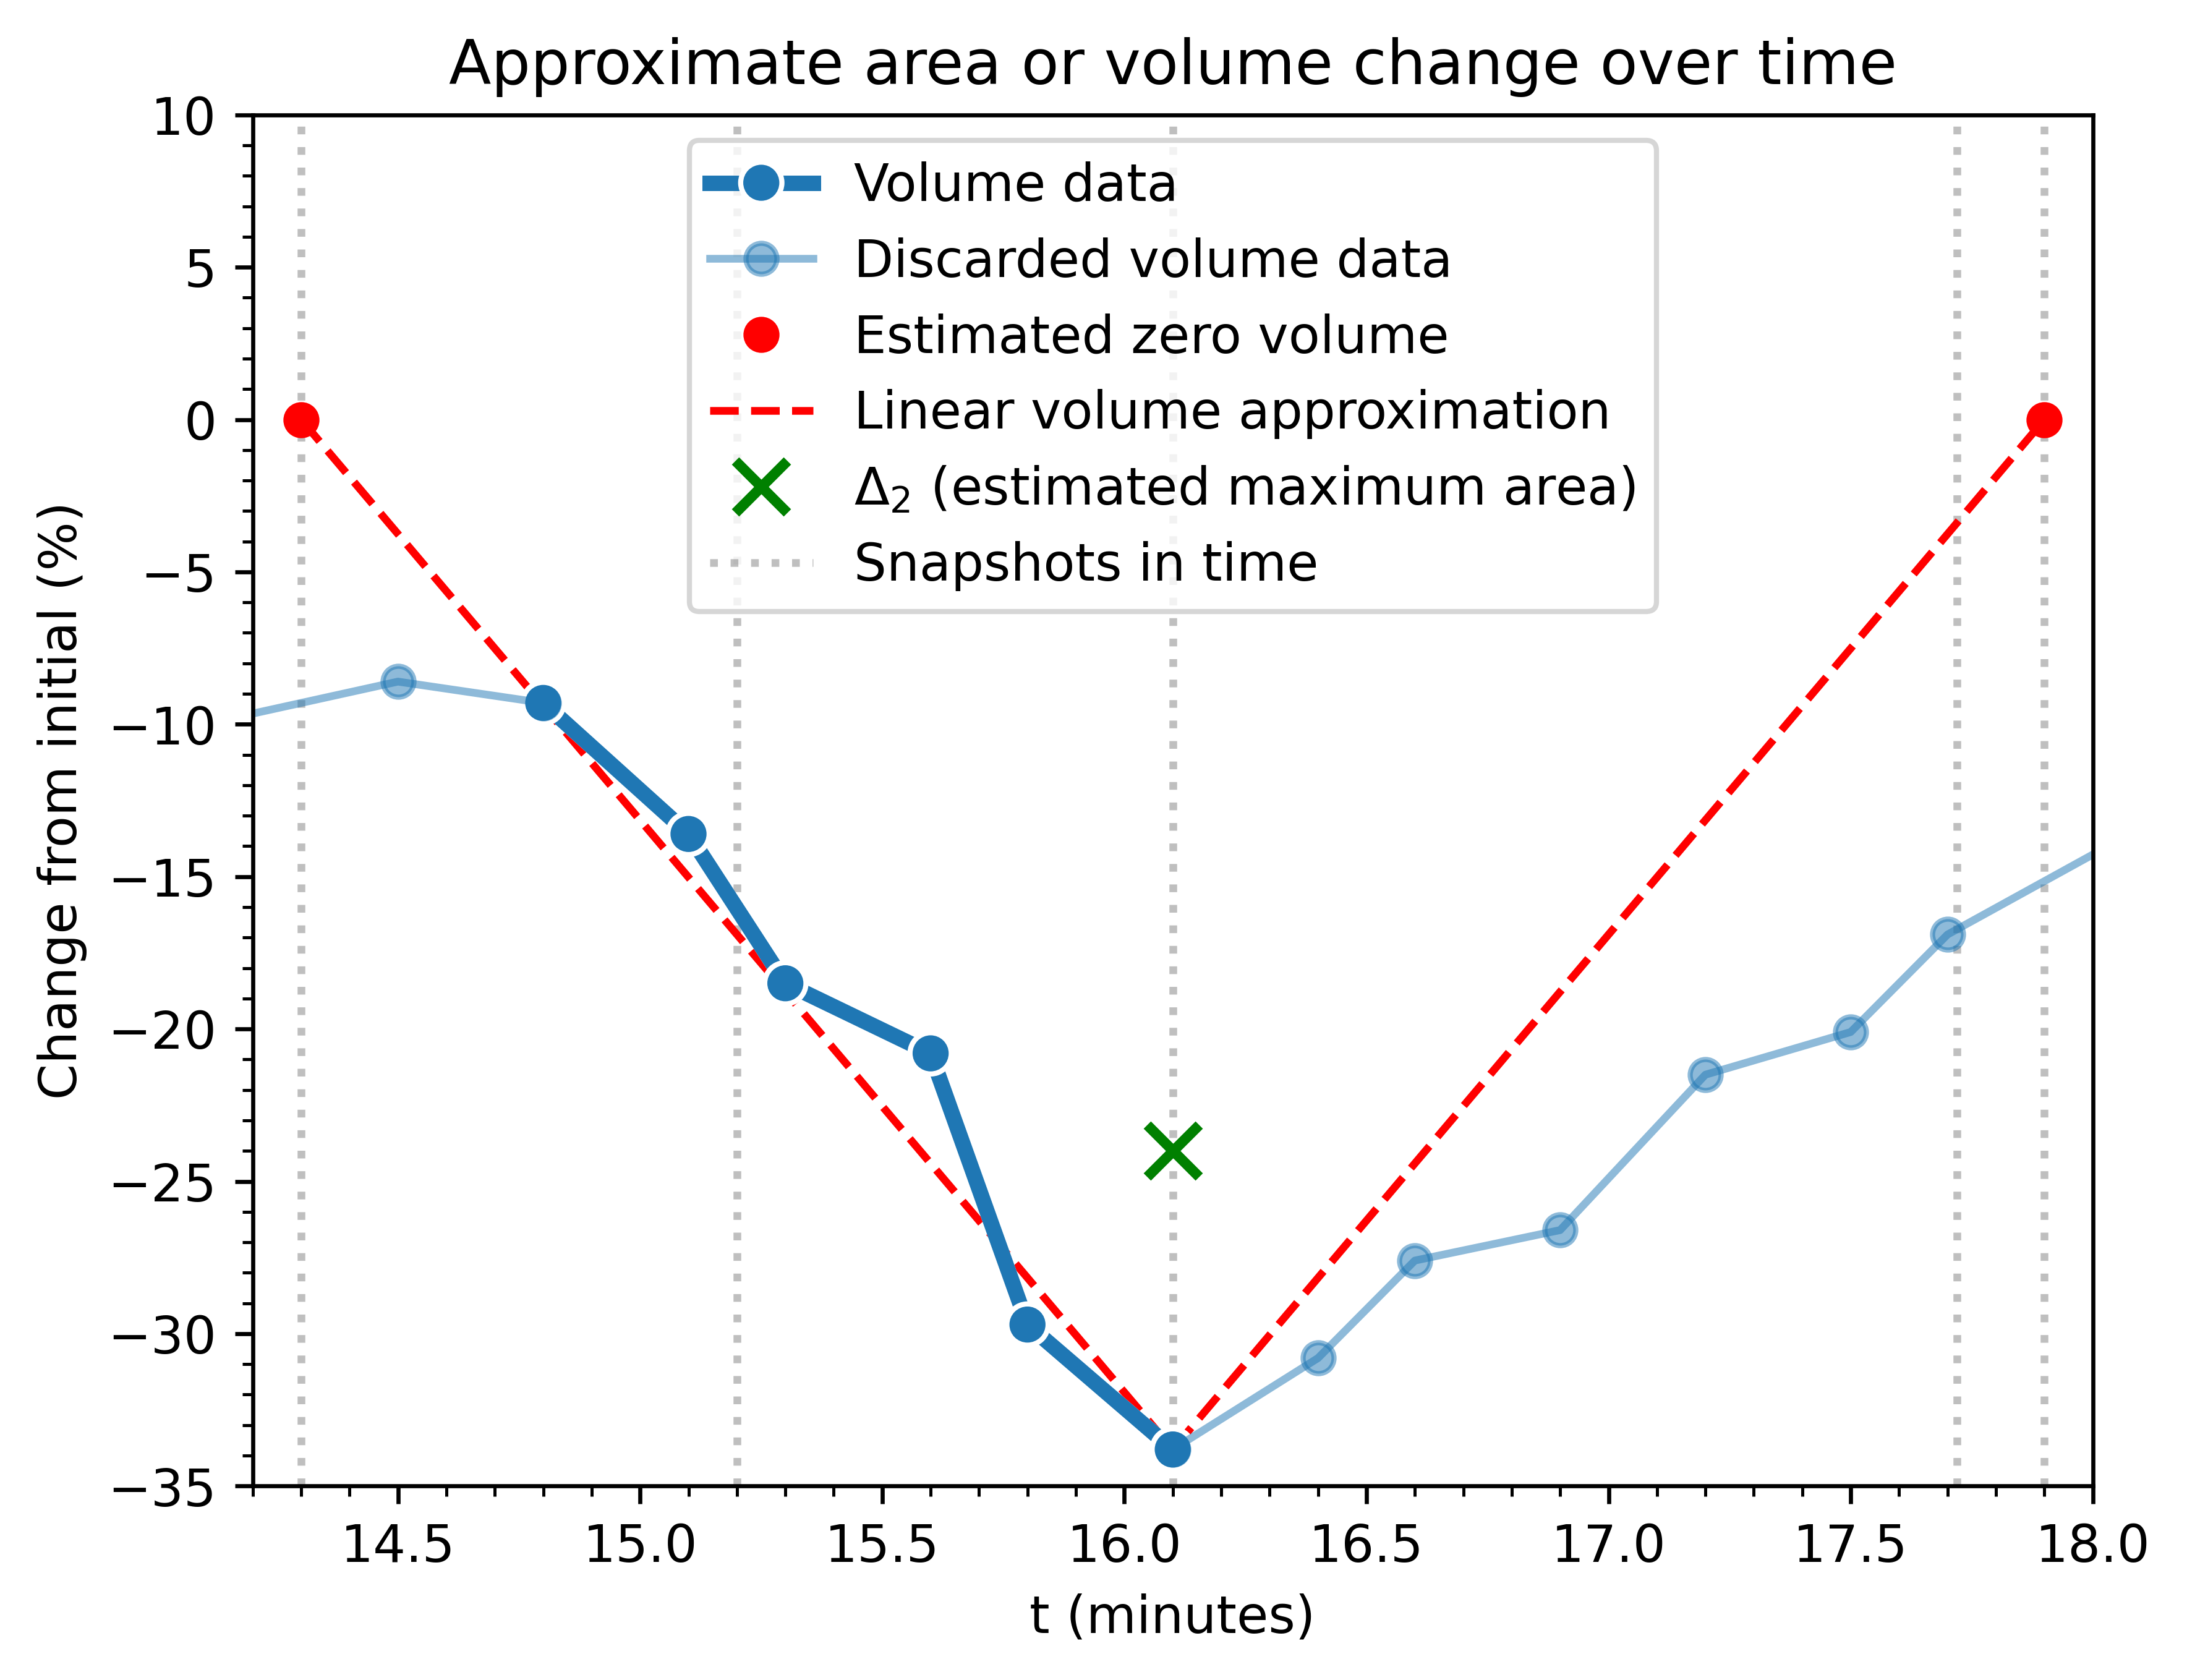
\includegraphics[width=0.75\textwidth]{diagrams/results-contractions/extracted-contraction-data.png}
                    \caption{}
                    \label{fig:contraction-data:extracted}
                \end{subfigure}
                \caption{(a) Graph taken from \citeauthor{gowlandCharacterisingPlacentalContractions2024} \cite{gowlandCharacterisingPlacentalContractions2024} and overlaid with a black box to indicate the region we are interested in modelling in this thesis. Specifically, this is the placental volume change during the period of fastest volume reduction of a placental contraction between approximately $15$ and $16$ minutes. (b) A simpler visualisation of (a) on the region of interest. \S\ref{sec:contractions:placenta:mesh-velocity} describes the simplifications we make of assuming a linear decrease in volume during the period of fastest volume decrease (indicated by the red dotted line), and an appropriate area decrease for an equivalent 2D area change for this 3D volume change (indicated by the green cross). We then assume that the areas and volumes increase at the same rate, back to their original sizes at $t = 17.9$ minutes. Grey vertical lines indicate the snapshots at which Figures \ref{fig:moving-mesh-placenta-velocity} and \ref{fig:moving-mesh-placenta-transport} are visualised.}
                \label{fig:contraction-data}
            \end{figure}
            
            For ease of presentation, we plot again the volume change data points in this region of interest in Figure \ref{fig:contraction-data:extracted}, plotted using blue lines. This shows the largest volume change of $-33.8\%$ at $t=16.1$ minutes. Prior to this, there is a roughly linear decrease in volume from $t=14.8$ minutes. Extrapolating the straight line passing through both of these points (red dotted line), we find the point at which this line meets the horizontal axis to be at $t = 14.3$ minutes (red dot). We make the assumption that the volume increase after a placental contraction is at the same rate as the volume decrease. We therefore model the contraction behaviour between $T_0:=14.3$ and $T_N:=17.9$ minutes, with maximum volume at times $T_0$ and $T_N$ minutes, and a minimum volume at $\frac{T_0+T_N}{2}=16.1$ minutes.

            A complication with using this data is that it concerns a 3D volume. We therefore need to calculate an analogous 2D area change to an equivalent 3D volume. Denoting percentage change in a 2D area by $\Delta_2$, and percentage change in 3D volume by $\Delta_3$, we assume for simplicity that the relationship between a 2D area change and 3D volume change is given through the following relationship:
            \begin{equation}
                (1 + \Delta_2)^{\frac{1}{2}} = (1 + \Delta_3)^{\frac{1}{3}}.
                \label{eq:2D-area-change-to-3D-volume-change}
            \end{equation}
            In our case, $\Delta_3 = -33.8\%$ at the smallest measured volume, which through Equation \eqref{eq:2D-area-change-to-3D-volume-change} gives a 2D area change of $\Delta_2 = -24.0\%$, which is indicated in Figure \ref{fig:contraction-data:extracted} with a green cross.

            Next, we prescribe a domain velocity. For simplicity, we assume that the placenta contracts uniformly in both directions and follows a sinusoidal speed through time. We therefore select the domain velocity $\vec{w} \equiv (w_1, w_2)^\intercal$ from \S\ref{sec:contractions:numerical-experiments:boundary-movement}:
            \begin{subequations}
                \begin{equation}
                    \retag{eq:oscillating-mesh-velocity:1}
                    w_1 = W (x - x_c) \sin\left(\frac{2 \pi t - T_0}{T}\right),
                \end{equation}
                \begin{equation}
                    \retag{eq:oscillating-mesh-velocity:2}
                    w_2 = W (y - y_c) \sin\left(\frac{2 \pi t - T_0}{T}\right),
                \end{equation}
            \end{subequations}
            where $(x_c, y_c)$ is selected as a centre of inflation within the 2D placenta, $T_0=14.3$ and $T = T_N - T_0 = 3.6$ minutes, and $W$ is chosen appropriately such that at time $\frac{T_0+T_N}{2}$ minutes there is a 2D area change of $\Delta_2 = -24.0\%$; here, this corresponds to $W = \qty{8.04e-5}{\metre\per\second}$.
            
            To summarise, we have used MRI scan data of placental volume change during a placental contraction to inform a domain velocity for use in our mathematical model. Specifically, we made a simplification to only consider the period of fastest volume decrease in this data, and calculated an equivalent area change for our 2D geometry from this 3D data. We then selected a simple form of domain velocity that gives an equivalent maximum area reduction on our 2D placenta geometry between $T_0 = 14.3$ and $T_N = 17.9$ minutes.

            We will now introduce the problem we aim to address.

        \subsection{Problem setup} \label{sec:contractions:placenta:problem-setup}
            Using the domain velocity from \S\ref{sec:contractions:placenta:mesh-velocity}, we will now specify the moving boundary problem we intend to compute approximations to.
            
            For the flow problem, we consider a small modification to the boundary conditions to those presented in \S\ref{sec:modelling:blood-flow:boundary-conditions}. We recall boundary conditions are applied in the form
            \begin{subequations}
                \begin{alignat*}{3}
                    \left( \nabla \vec{u} - p \mat{I} \right) \cdot \vec{n} & = \vec{g}_\text{f,N} &&~ \text{on } \Gamma_\text{out}, \\
                    \vec{u} & = \vec{g}_\text{f,D} &&~ \text{on } \Gamma\setminus\Gamma_\text{out},
                \end{alignat*}%
            \end{subequations}%
            and we select these boundary condition functions such that there is a zero Neumann condition on outflow, a parabolic inflow velocity profile, and no velocity slip elsewhere. We additionally choose the amplitude of this parabolic inflow such that the flux of incoming blood is constant through time. We note that, in order to impose no-slip boundary conditions on solid walls, the velocity must take the value of the domain velocity $\vec{w}$ at the boundary. The modified boundary conditions for this moving boundary problem are given by
            \begin{subequations}
                \begin{alignat}{3}
                    \vec{g}_\text{f,D} & = - A(t) \frac{R(t)^2 - r^2}{R(t)^2} \vec{n} &&~ \text{on } \Gamma_\text{in}, \\
                    \vec{g}_\text{f,N} & = \vec{0} &&~ \text{on } \Gamma_\text{out},\\
                    \vec{g}_\text{f,D} & = \vec{w} &&~ \text{on } \Gamma \setminus (\Gamma_\text{in} \cup \Gamma_\text{out}),
                \end{alignat}%
            \end{subequations}%
            where $\vec{n}$ is the unit outward-pointing normal on $\Gamma_\text{in}$, $r(\vec{x})$ is the distance from a point $\vec{x}$ to the centre of $\Gamma_\text{in}$, $R(t)$ is the artery radius, and $A(t) := \frac{R(0)}{R(t)}$ is the modified amplitude of the Poiseuille flow to retain constant inlet flux.

            For the oxygen transport problem, we keep the same boundary conditions as those presented in \S\ref{sec:modelling:transport}; namely, boundary conditions are applied of the form
            \begin{subequations}
                \begin{alignat*}{3}
                    c & = g_\text{c,D} &&~ \text{on } \Gamma_\text{in}, \\
                    \nabla c \cdot \vec{n} & = g_\text{c,N} &&~ \text{on } \Gamma\setminus\Gamma_\text{in},
                \end{alignat*}%
            \end{subequations}
            and the boundary condition functions are given as
            \begin{subequations}
                \begin{alignat}{3}
                    g_\text{c,D} & = 1 &&~ \text{on } \Gamma_\text{in},\retag{eq:oxygen-bcs:dirichlet}\\
                    g_\text{c,N} & = 0 &&~ \text{on } \Gamma\setminus\Gamma_\text{in}.\retag{eq:oxygen-bcs:neumann}%
                \end{alignat}%
            \end{subequations}%

            We will now use the prescribed domain velocity from \S\ref{sec:contractions:placenta:mesh-velocity} and the problem setup presented here, together with the numerical methods from \S\ref{sec:contractions:dgfem-discretisation}, to compute the blood flow and oxygen transport fields under this domain movement.

        \subsection{Placenta motion}
            We take our initial domain $\Omega^0$ to be the 2D placenta domain with dimensions specified in \S\ref{sec:modelling:geometries:2d-placenta} and asymmetric placement of vessels as presented in \S\ref{sec:numerical-methods:blood-flow-experiments:asymmetric}. We use the steady-state approximations on $\Omega^0$ as the initial conditions for the time-dependent blood flow and oxygen concentration problems. For these simulations, we have selected a time-step size of $\Delta t = \qty{0.036}{\minute} = \qty{2.16}{\second}$. We note that each time-step is longer than a typical cardiac cycle, and we therefore do not apply any corresponding adjustment to the amplitude to account for pulsatile inlet flow. We chose this relatively large time-step size for simplicity, and because of the relatively slow domain velocity scaling of $W = \qty{8.04e-5}{\metre\per\second}$.

            We will consider only five snapshots in time in the body of this thesis for ease of presentation. Videos visualising these fields through time at every time-step are available here\footnote{Blood flow field: \url{https://r.blakey.family/phd-video-mmv}; oxygen transport field: \url{https://r.blakey.family/phd-video-mmt}}. Figures \ref{fig:moving-mesh-placenta-velocity} and \ref{fig:moving-mesh-placenta-transport} provide the main results of this chapter. These figures respectively visualise the blood flow and oxygen transport fields in five snapshots in time, which are indicated in Figure \ref{fig:contraction-data:extracted} by grey vertical lines.

            \begin{figure}
                \centering
                \begin{subfigure}{\textwidth}
                    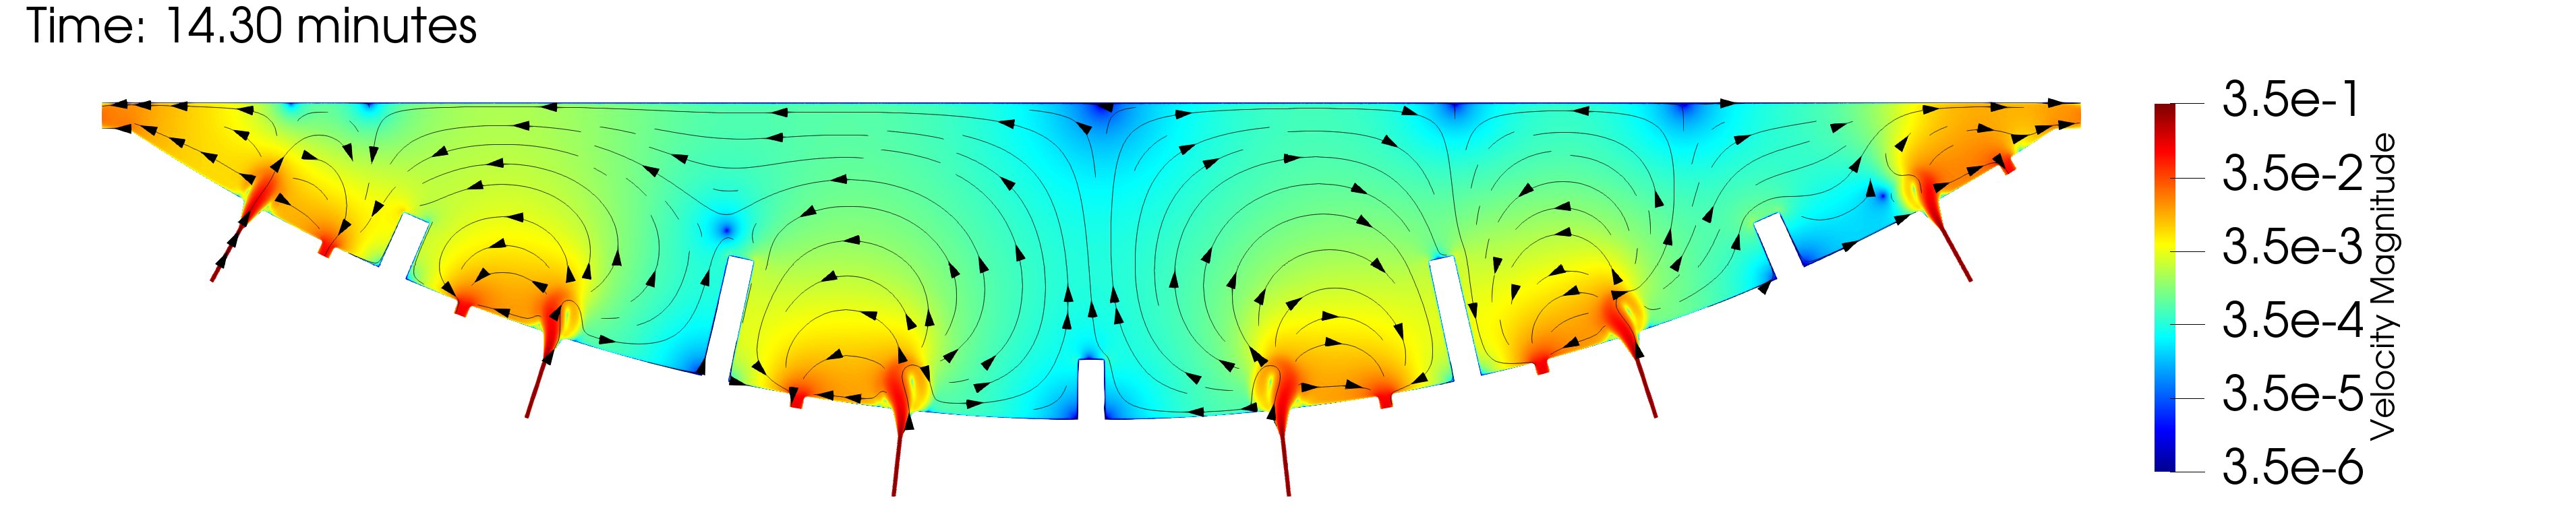
\includegraphics[width=\textwidth]{diagrams/results-contractions/placenta-moving-mesh/mm-placenta-velocity.0000.png}
                    \caption{}
                    \label{fig:moving-mesh-placenta-velocity:1}
                \end{subfigure}
                \begin{subfigure}{\textwidth}
                    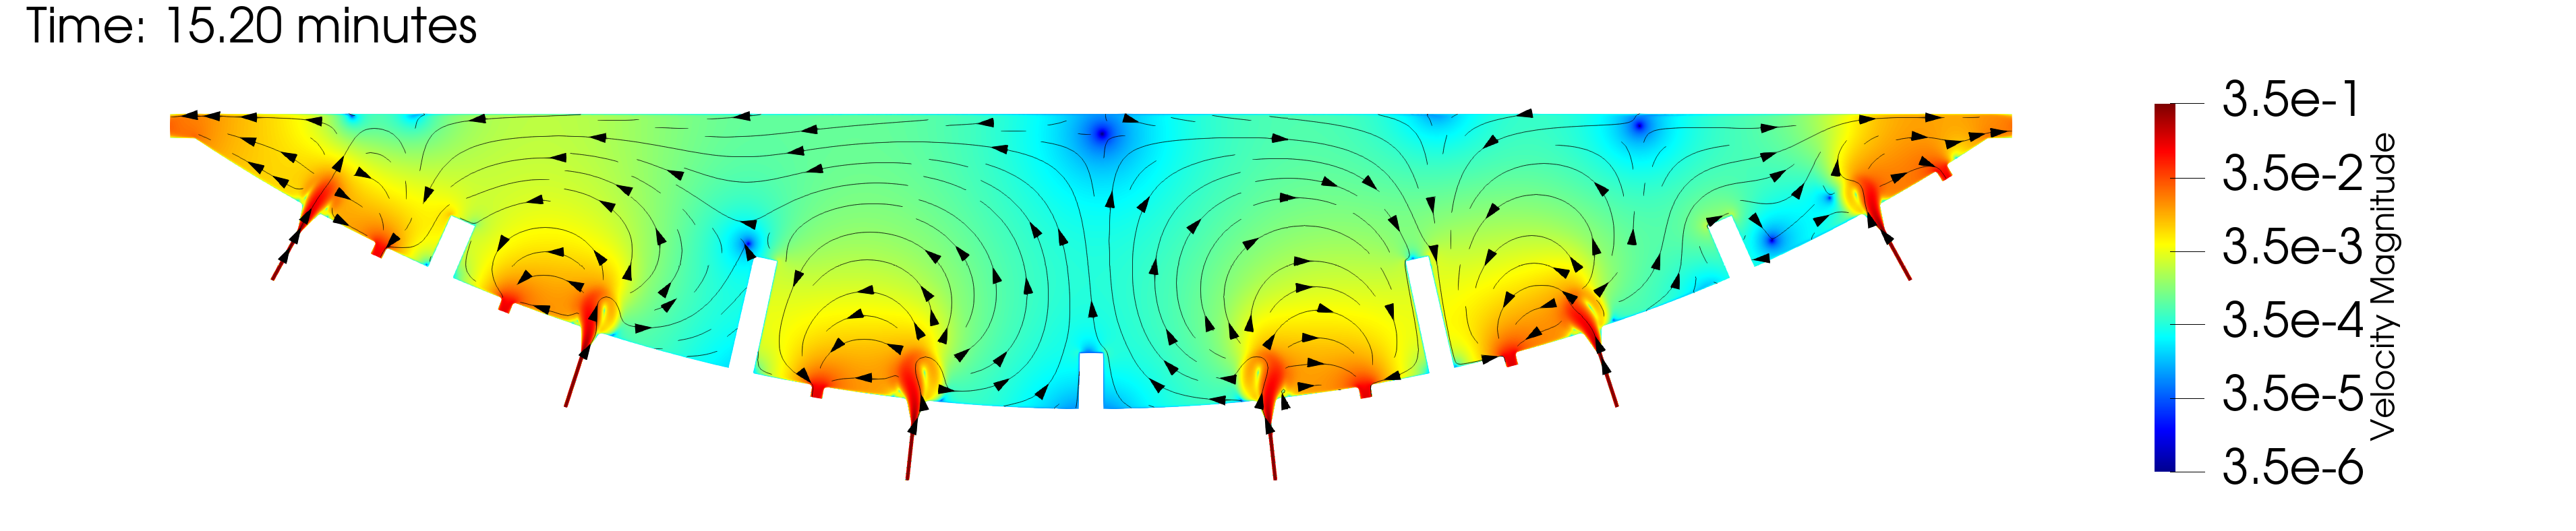
\includegraphics[width=\textwidth]{diagrams/results-contractions/placenta-moving-mesh/mm-placenta-velocity.0025.png}
                    \caption{}
                    \label{fig:moving-mesh-placenta-velocity:2}
                \end{subfigure}
                \begin{subfigure}{\textwidth}
                    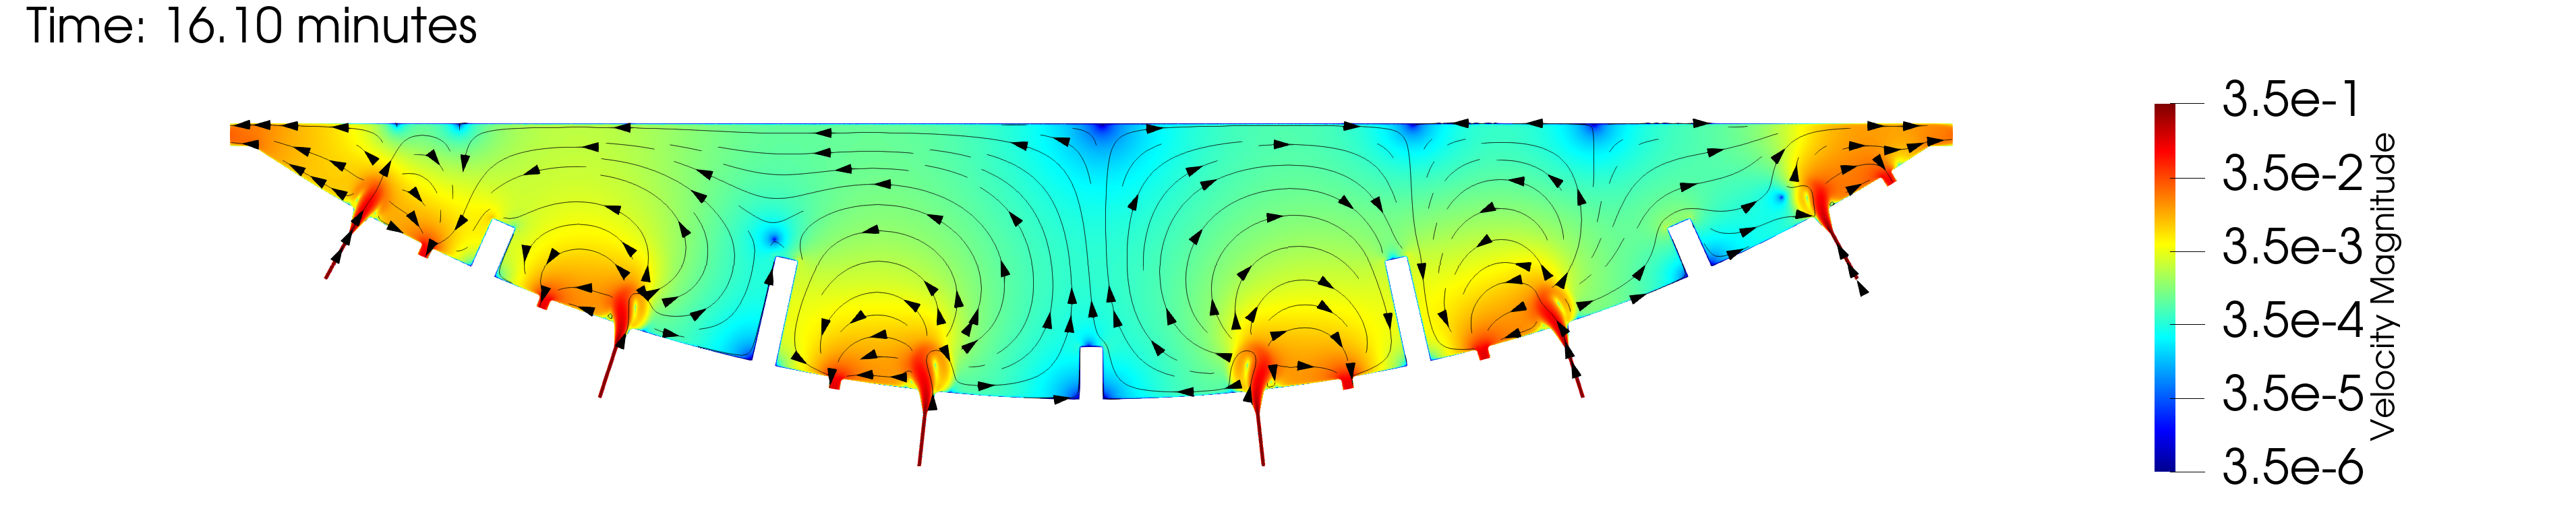
\includegraphics[width=\textwidth]{diagrams/results-contractions/placenta-moving-mesh/mm-placenta-velocity.0050.png}
                    \caption{}
                    \label{fig:moving-mesh-placenta-velocity:3}
                \end{subfigure}
                \begin{subfigure}{\textwidth}
                    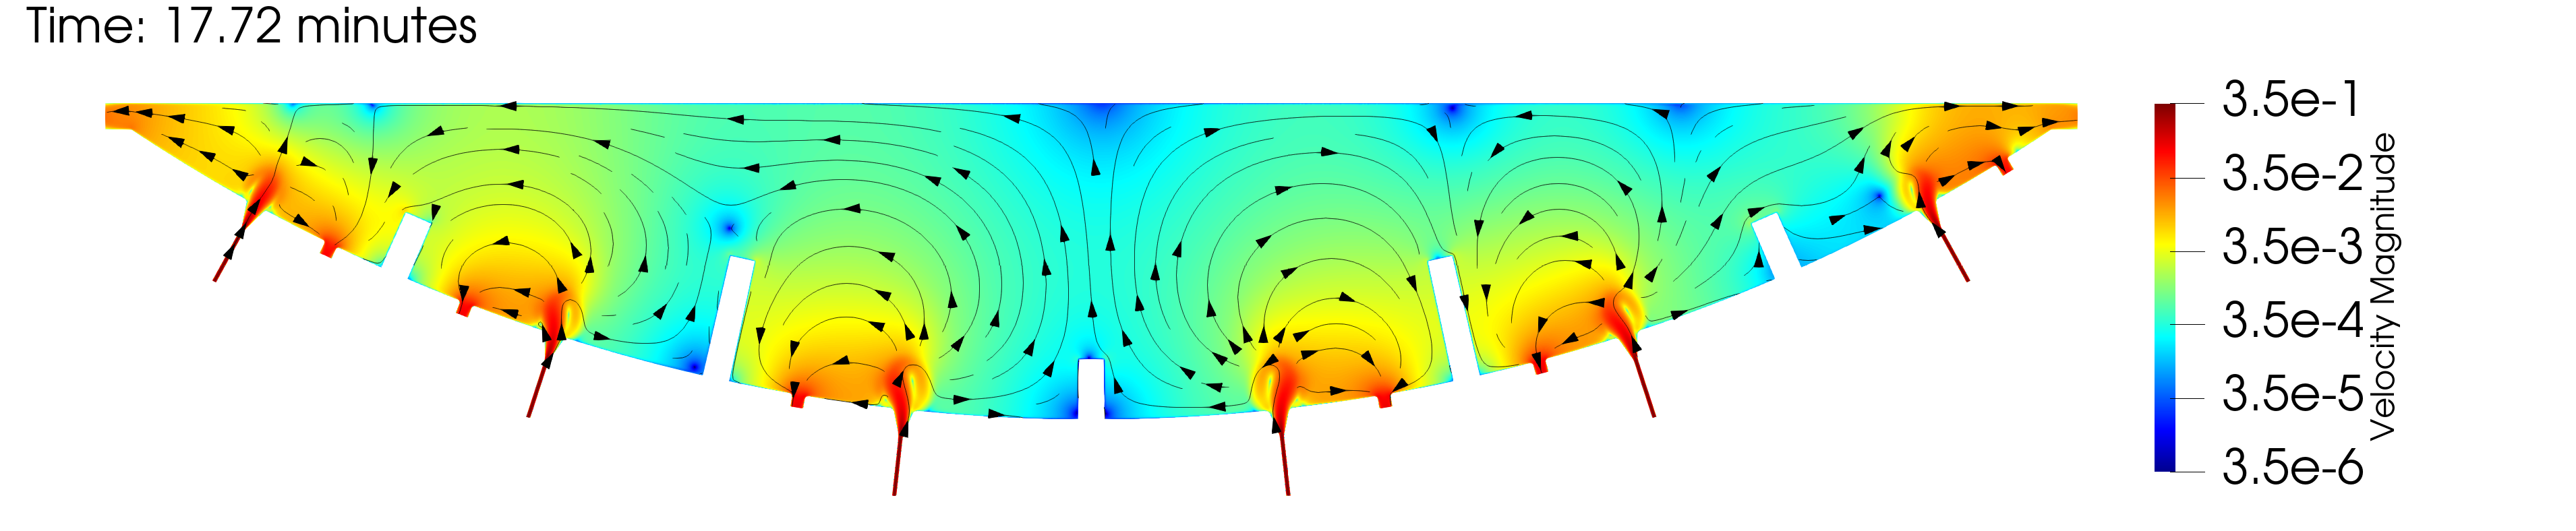
\includegraphics[width=\textwidth]{diagrams/results-contractions/placenta-moving-mesh/mm-placenta-velocity.0095.png}
                    \caption{}
                    \label{fig:moving-mesh-placenta-velocity:4}
                \end{subfigure}
                \begin{subfigure}{\textwidth}
                    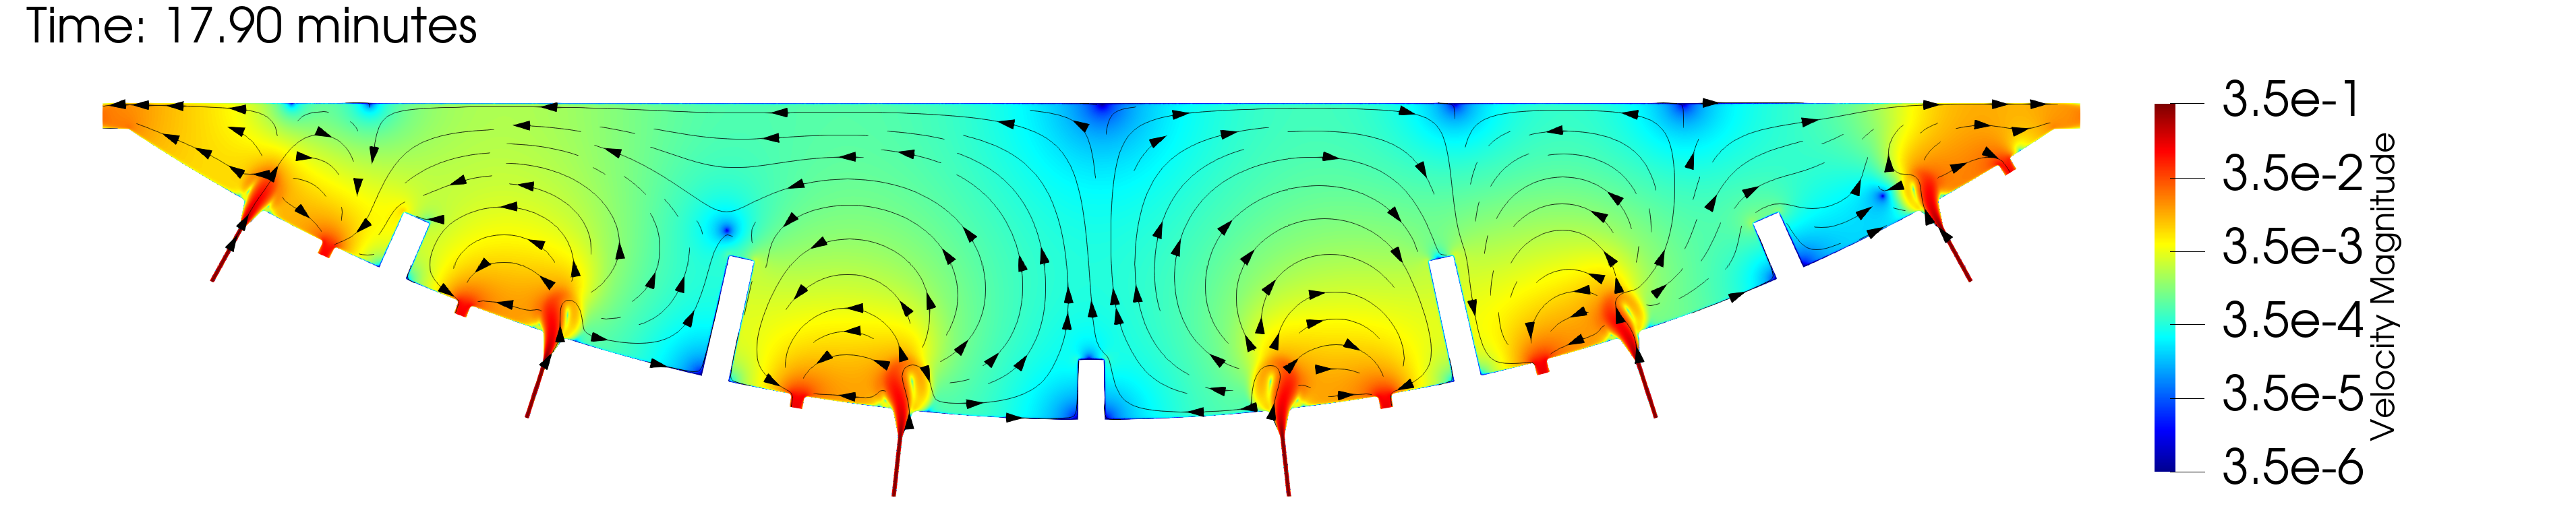
\includegraphics[width=\textwidth]{diagrams/results-contractions/placenta-moving-mesh/mm-placenta-velocity.0100.png}
                    \caption{}
                    \label{fig:moving-mesh-placenta-velocity:5}
                \end{subfigure}
                \caption{Visualisation of the blood flow field during a contraction at times (a) $t=\qty{14.30}{\minute}$, (b) $t=\qty{15.20}{\minute}$, (c) $t=\qty{16.10}{\minute}$, (d) $t=\qty{17.72}{\minute}$, and (e) $t=\qty{17.9}{\minute}$. Colours are logarithmically scaled, and streamlines at each time-step are shown with black lines. A video visualising all time-steps can be viewed here: \url{https://r.blakey.family/phd-video-mmv}}
                \label{fig:moving-mesh-placenta-velocity}
            \end{figure}

            \begin{figure}
                \centering
                \begin{subfigure}{\textwidth}
                    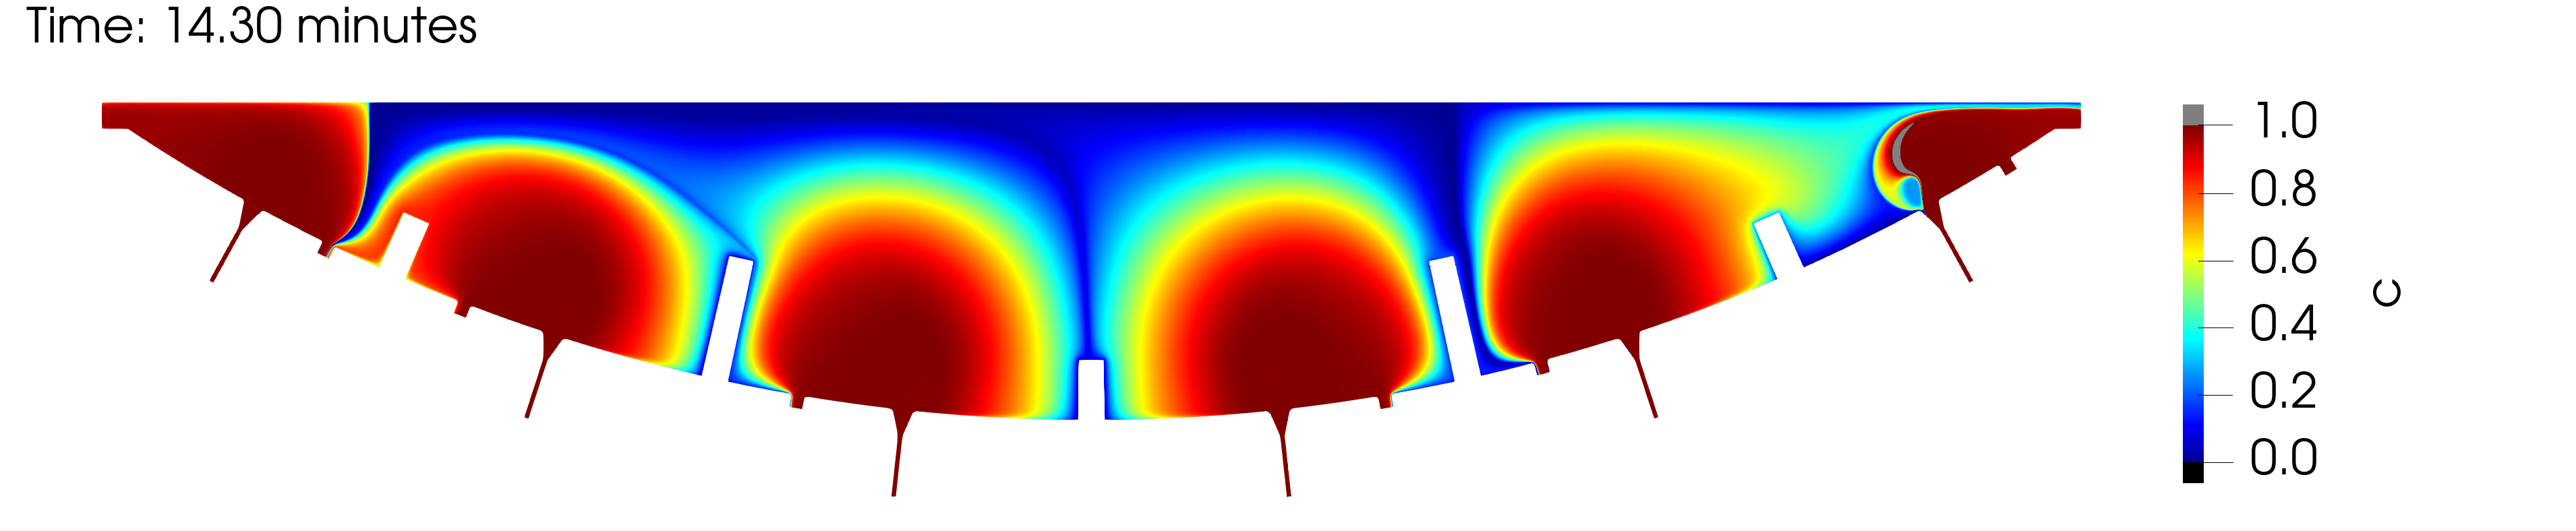
\includegraphics[width=\textwidth]{diagrams/results-contractions/placenta-moving-mesh/mm-placenta-transport.0000.png}
                    \caption{}
                    \label{fig:moving-mesh-placenta-transport:1}
                \end{subfigure}
                \begin{subfigure}{\textwidth}
                    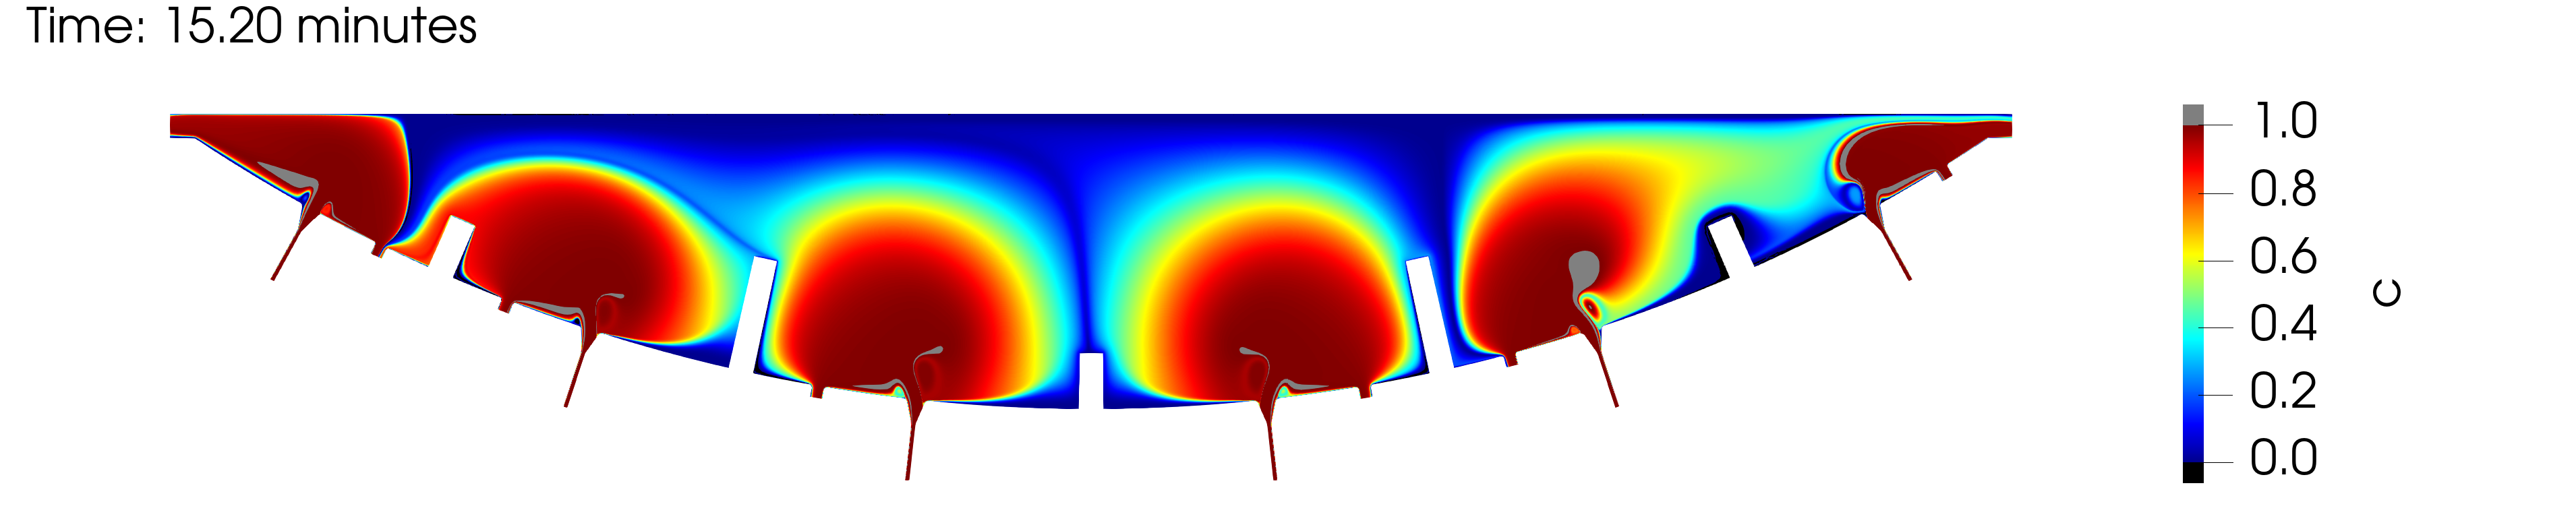
\includegraphics[width=\textwidth]{diagrams/results-contractions/placenta-moving-mesh/mm-placenta-transport.0025.png}
                    \caption{}
                    \label{fig:moving-mesh-placenta-transport:2}
                \end{subfigure}
                \begin{subfigure}{\textwidth}
                    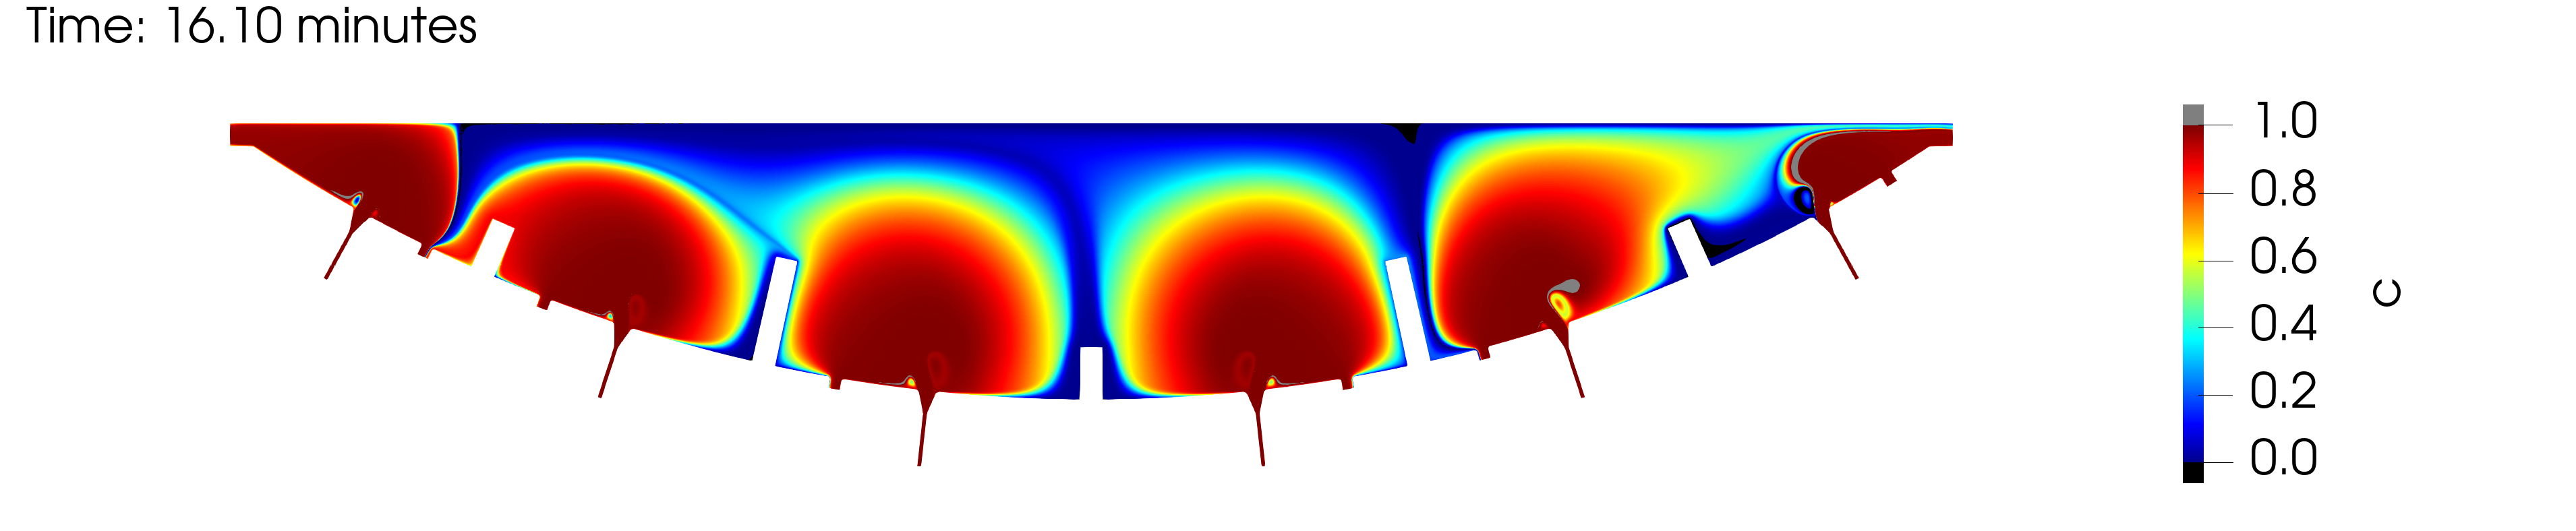
\includegraphics[width=\textwidth]{diagrams/results-contractions/placenta-moving-mesh/mm-placenta-transport.0050.png}
                    \caption{}
                    \label{fig:moving-mesh-placenta-transport:3}
                \end{subfigure}
                \begin{subfigure}{\textwidth}
                    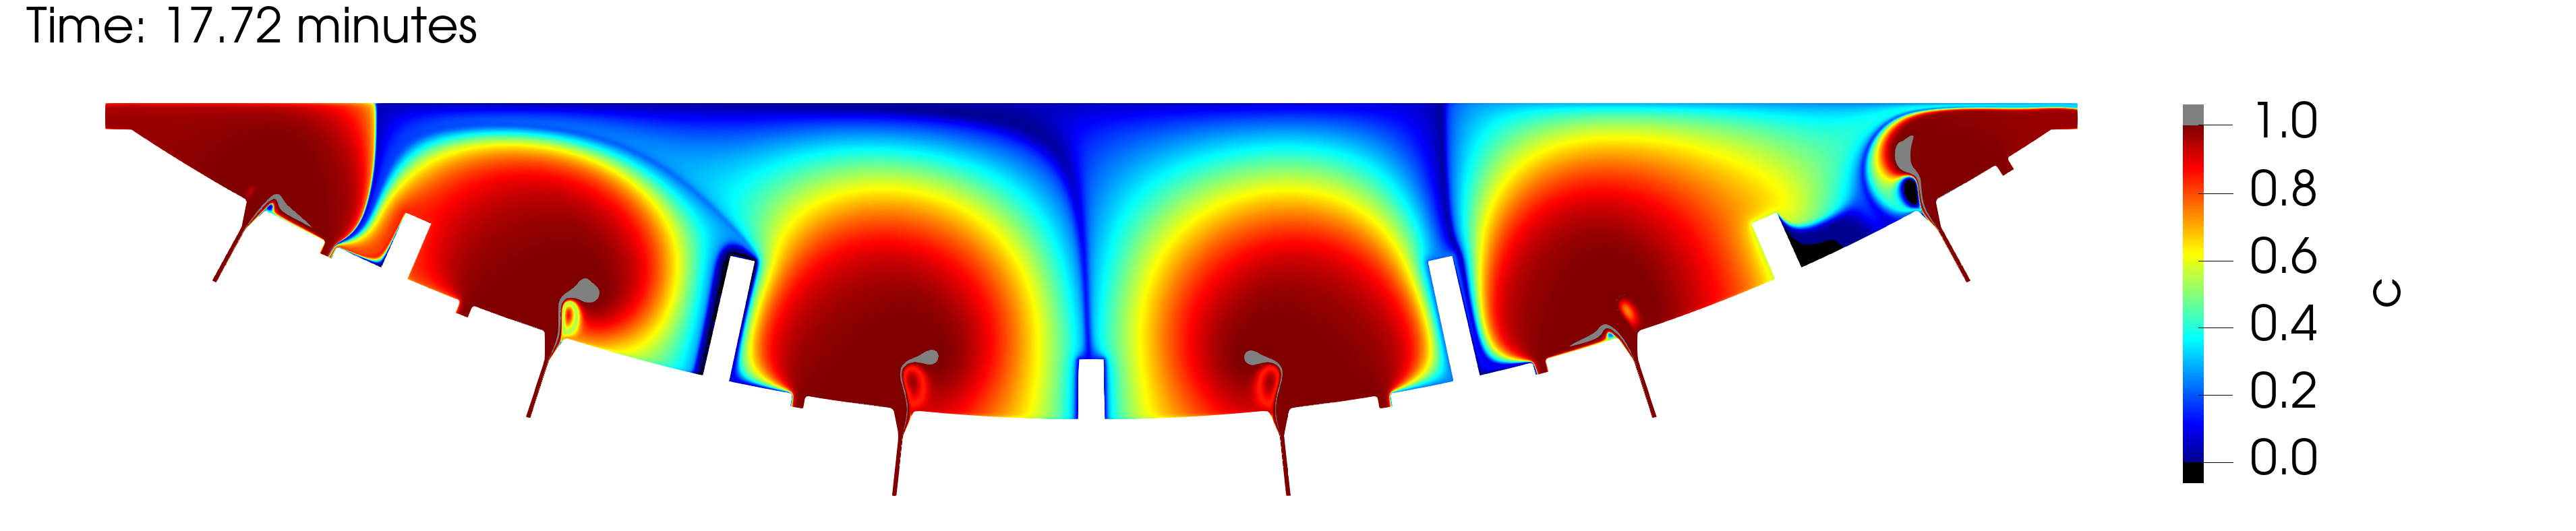
\includegraphics[width=\textwidth]{diagrams/results-contractions/placenta-moving-mesh/mm-placenta-transport.0095.png}
                    \caption{}
                    \label{fig:moving-mesh-placenta-transport:4}
                \end{subfigure}
                \begin{subfigure}{\textwidth}
                    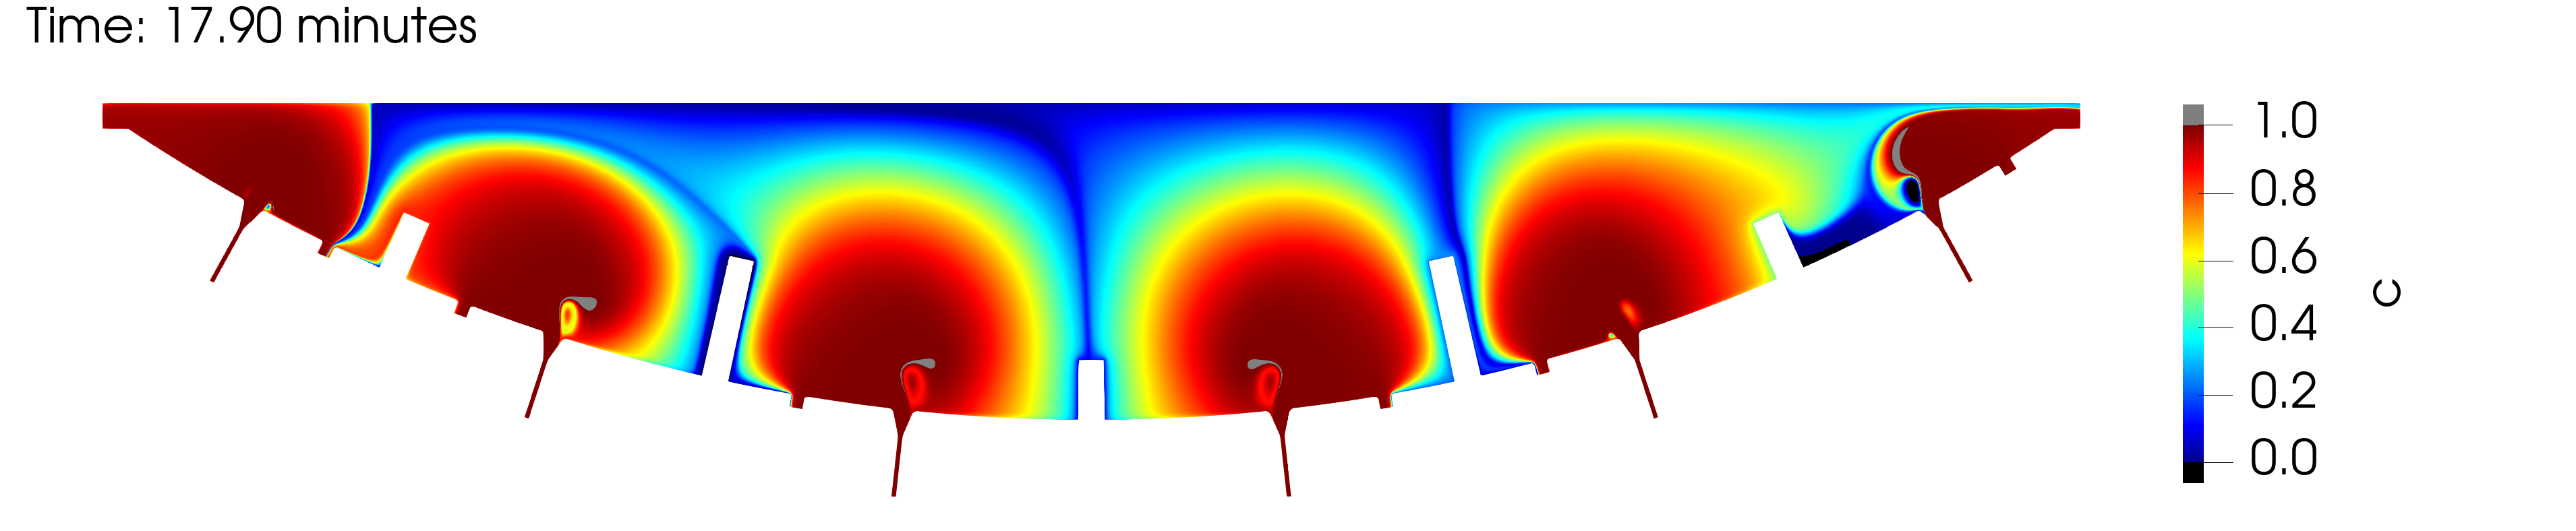
\includegraphics[width=\textwidth]{diagrams/results-contractions/placenta-moving-mesh/mm-placenta-transport.0100.png}
                    \caption{}
                    \label{fig:moving-mesh-placenta-transport:5}
                \end{subfigure}
                \caption{Visualisation of the oxygen concentration field during a contraction at times (a) $t=\qty{14.30}{\minute}$, (b) $t=\qty{15.20}{\minute}$, (c) $t=\qty{16.10}{\minute}$, (d) $t=\qty{17.72}{\minute}$, and (e) $t=\qty{17.9}{\minute}$. Colours are linearly scaled. A video visualising all time-steps can be viewed here: \url{https://r.blakey.family/phd-video-mmt}}
                \label{fig:moving-mesh-placenta-transport}
            \end{figure}

            Panel (a) of Figures \ref{fig:moving-mesh-placenta-velocity} and \ref{fig:moving-mesh-placenta-transport} give the initial steady-state fields of the flow and oxygen concentration, respectively; we remark that these fields are identical to the fields presented in \S\ref{sec:numerical-methods:blood-flow-experiments:asymmetric} and \S\ref{sec:numerical-methods:time-dependent-experiments}.
            
            Despite the varying domain size, the blood flow field changes very little from the steady-state solution as time progresses, with only small changes in the slower regions of the domain; an example of a small change in flow is shown in Figure \ref{fig:moving-mesh-placenta-velocity:2}, where previously slow blood near septal walls is advected by the moving boundary at a slightly higher speed.
            
            On the other hand, the oxygen concentration field changes noticeably more, with clear changes in the solution between each of the five snapshots in time. Figure \ref{fig:moving-mesh-placenta-transport:2} shows the oxygen concentration field at time $t = T_0 + \frac{T}{4}$, which corresponds to the point of fastest domain decrease due to the sinusoidal domain velocity. Here, we see oxygen advected away from the basal plate, leaving small regions on the basal plate where no oxygen is present. It is interesting to see in this snapshot that there is a change near recirculation zones in the central cavities, where high concentrations of oxygen become encircled by lower concentration oxygen. As the oxygen concentration field evolves from Figure \ref{fig:moving-mesh-placenta-transport:1} to Figure \ref{fig:moving-mesh-placenta-transport:3}, the furthest right placentone contains a region to the left of the artery where oxygen concentration reduces over time; this is because oxygen is uptaken by the villous tree here and oxygen is not being replaced. As time progresses and the domain enlarges to Figure \ref{fig:moving-mesh-placenta-transport:5}, this region is again filled with oxygen.

            Overall, the oxygen concentration appears to decrease whilst the domain contracts, and appears to fill more of the domain in higher concentration during the latter domain expansion. To solidify our understanding of this and the effect on flow speed, we measure both the average speed and the uptake by the villous tree at each instant in time. Although each of the two previous chapters are distinct from the work presented here, we restate two of the efficiency measures from Chapter \ref{sec:nutrient-uptake}, which respectively give instantaneous measures of the speed and amount of oxygen uptaken by the entire villous tree:
            \begin{align}
                \bar{v}(\Omega) & := \frac{1}{|\Omega|} \int_{\Omega} |\vec{u}| \diff \vec{x}, \retag{eq:eff-v} \\
                \bar{c} & := \frac{R}{|\Omega|} \int_\Omega \Psi c \diff \vec{x}, \retag{eq:eff-c}
            \end{align}
            where $\vec{u}$ is the velocity of the blood flow, $c$ is the oxygen concentration field, $|\Omega| := \int_\Omega \diff \vec{x}$, $R$ is the uptake rate of the villous tree from Table \ref{tab:problem-parameters}, and $\Psi$ defines the smooth transition region described in \S\ref{sec:modelling:blood-flow}. Figures \ref{fig:mm-quantities:velocity} and \ref{fig:mm-quantities:uptake} respectively visualise $\bar{v}(\Omega)$ and $\bar{c}$ through our simulation.

            \begin{figure}
                %% MONOLITH COMMIT:
                %% File run: ./plotting/mm-quantities.py
                %% Date run: 2024-05-10 12:33:00
                \centering
                \begin{subfigure}{0.45\textwidth}
                    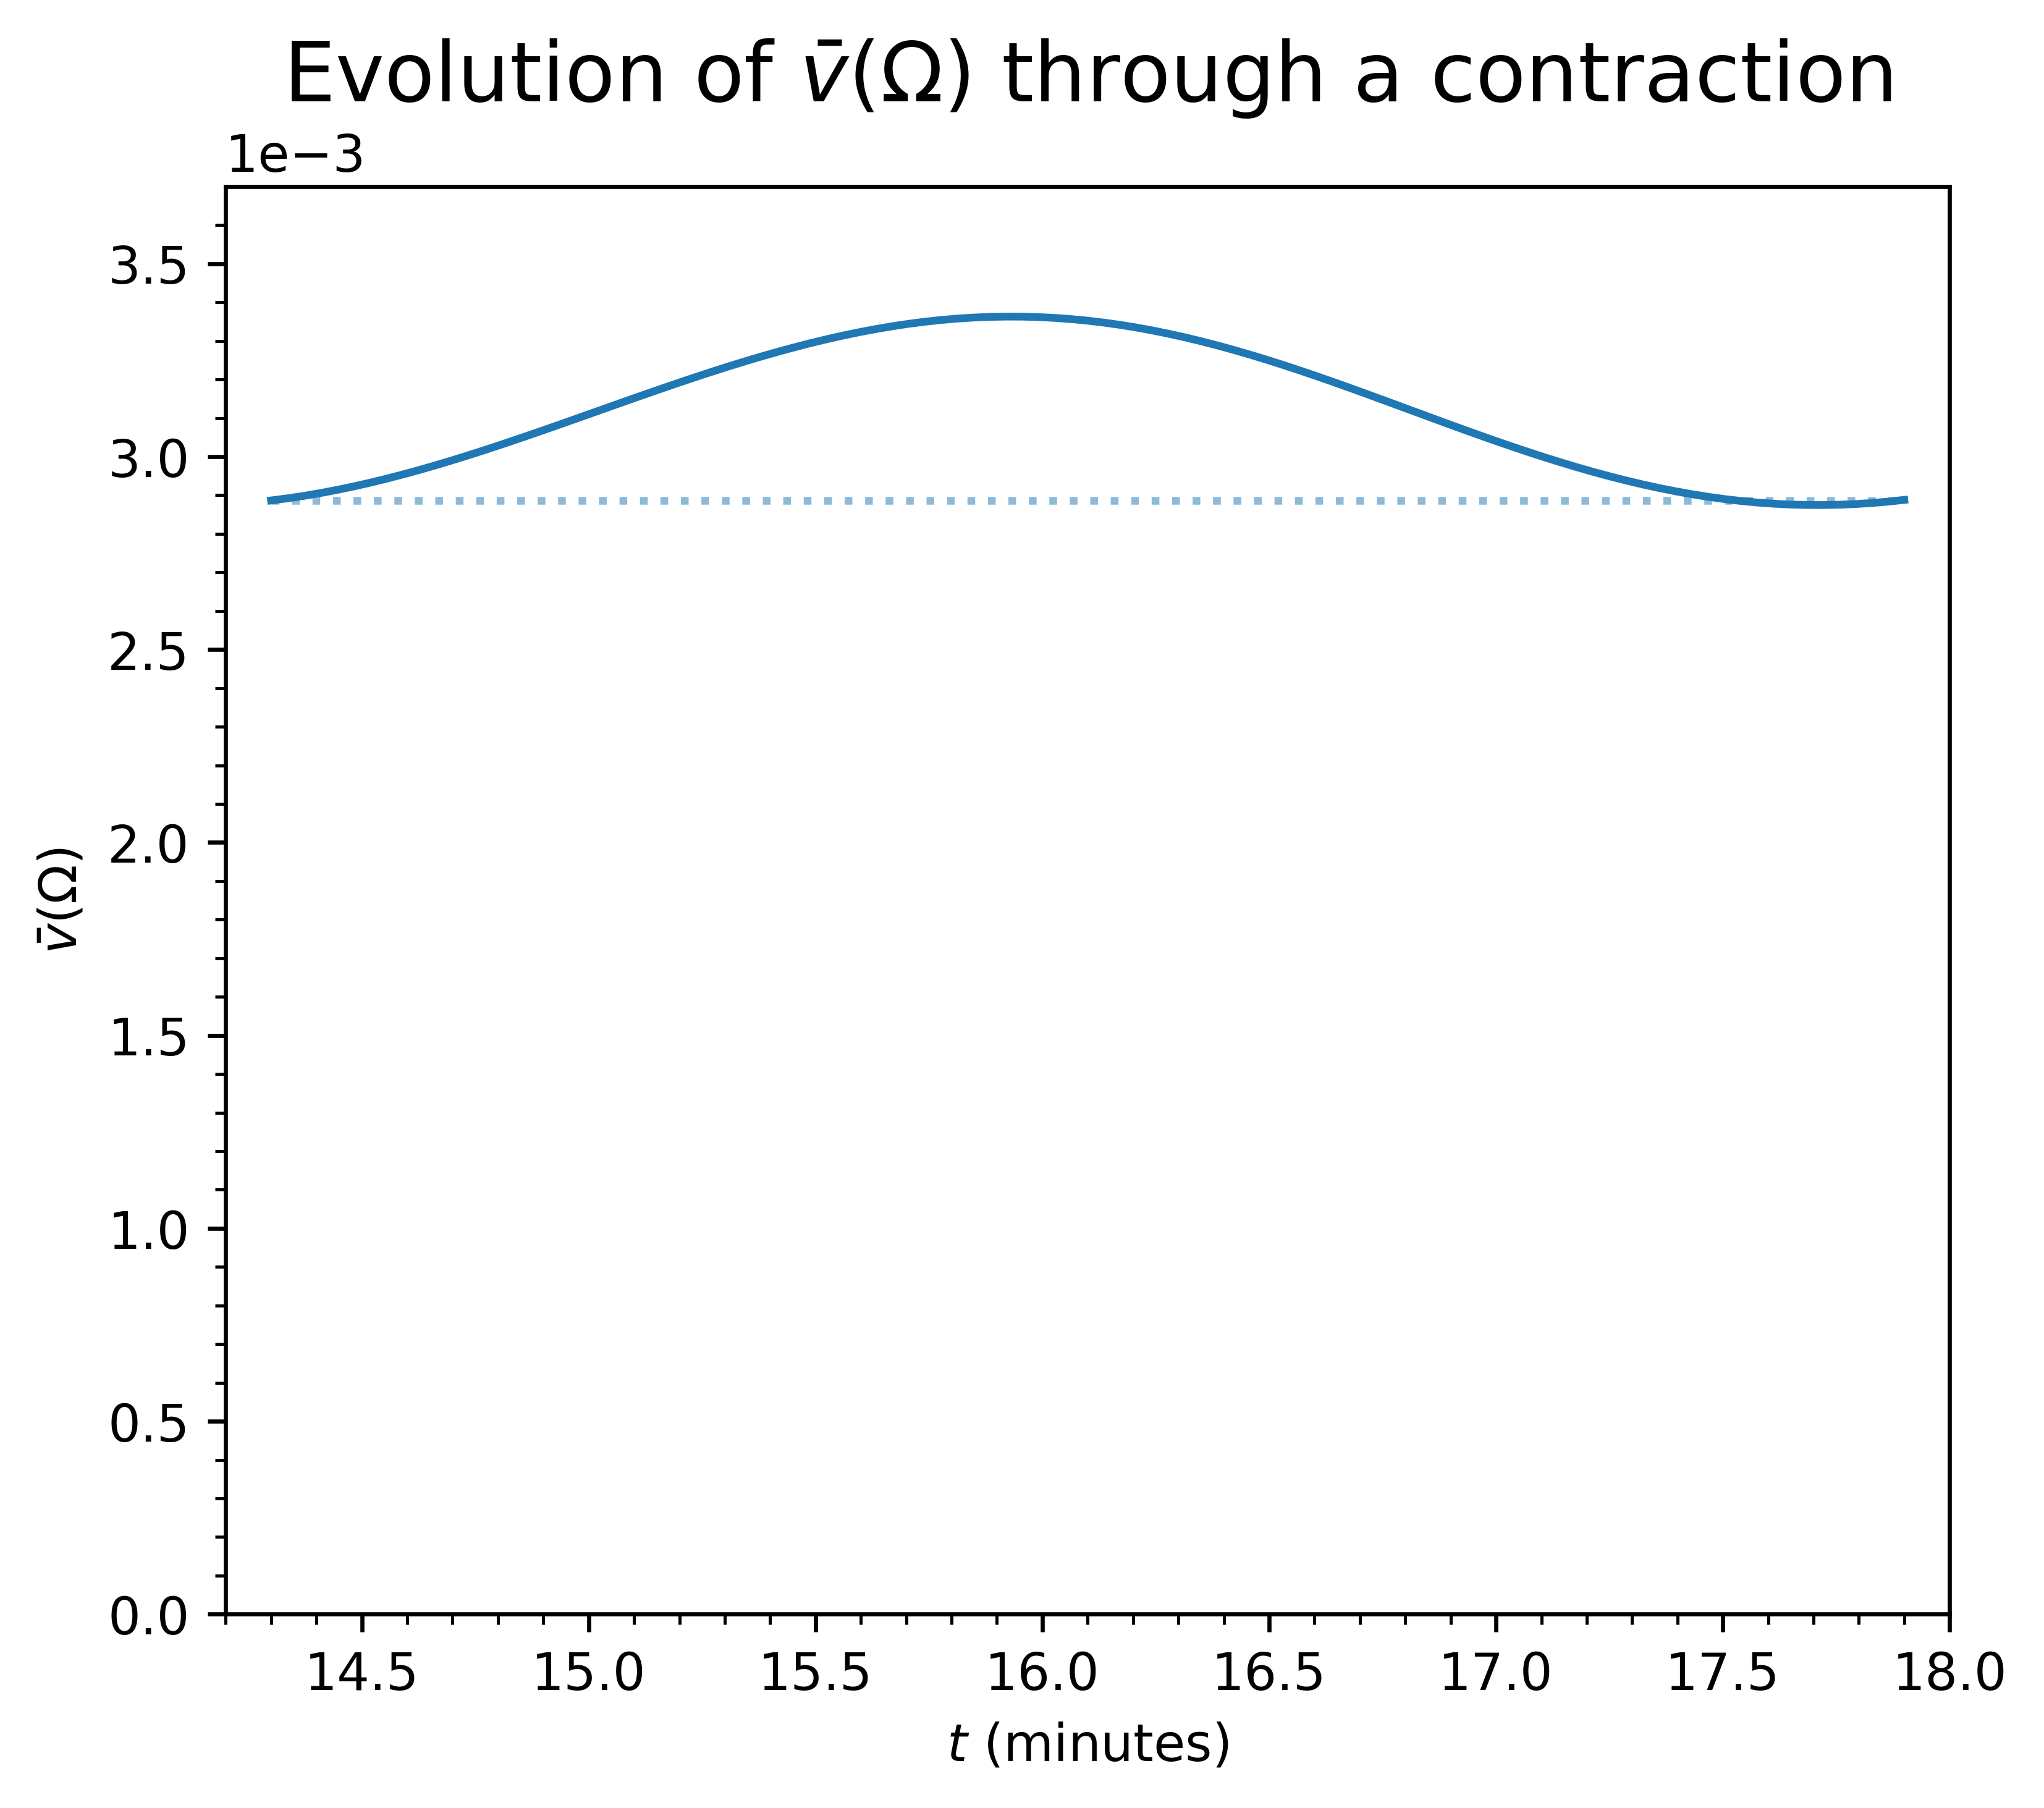
\includegraphics[width=\textwidth]{diagrams/results-contractions/mm-quantities-velocity.png}
                    \caption{}
                    \label{fig:mm-quantities:velocity}
                \end{subfigure}
                \begin{subfigure}{0.45\textwidth}
                    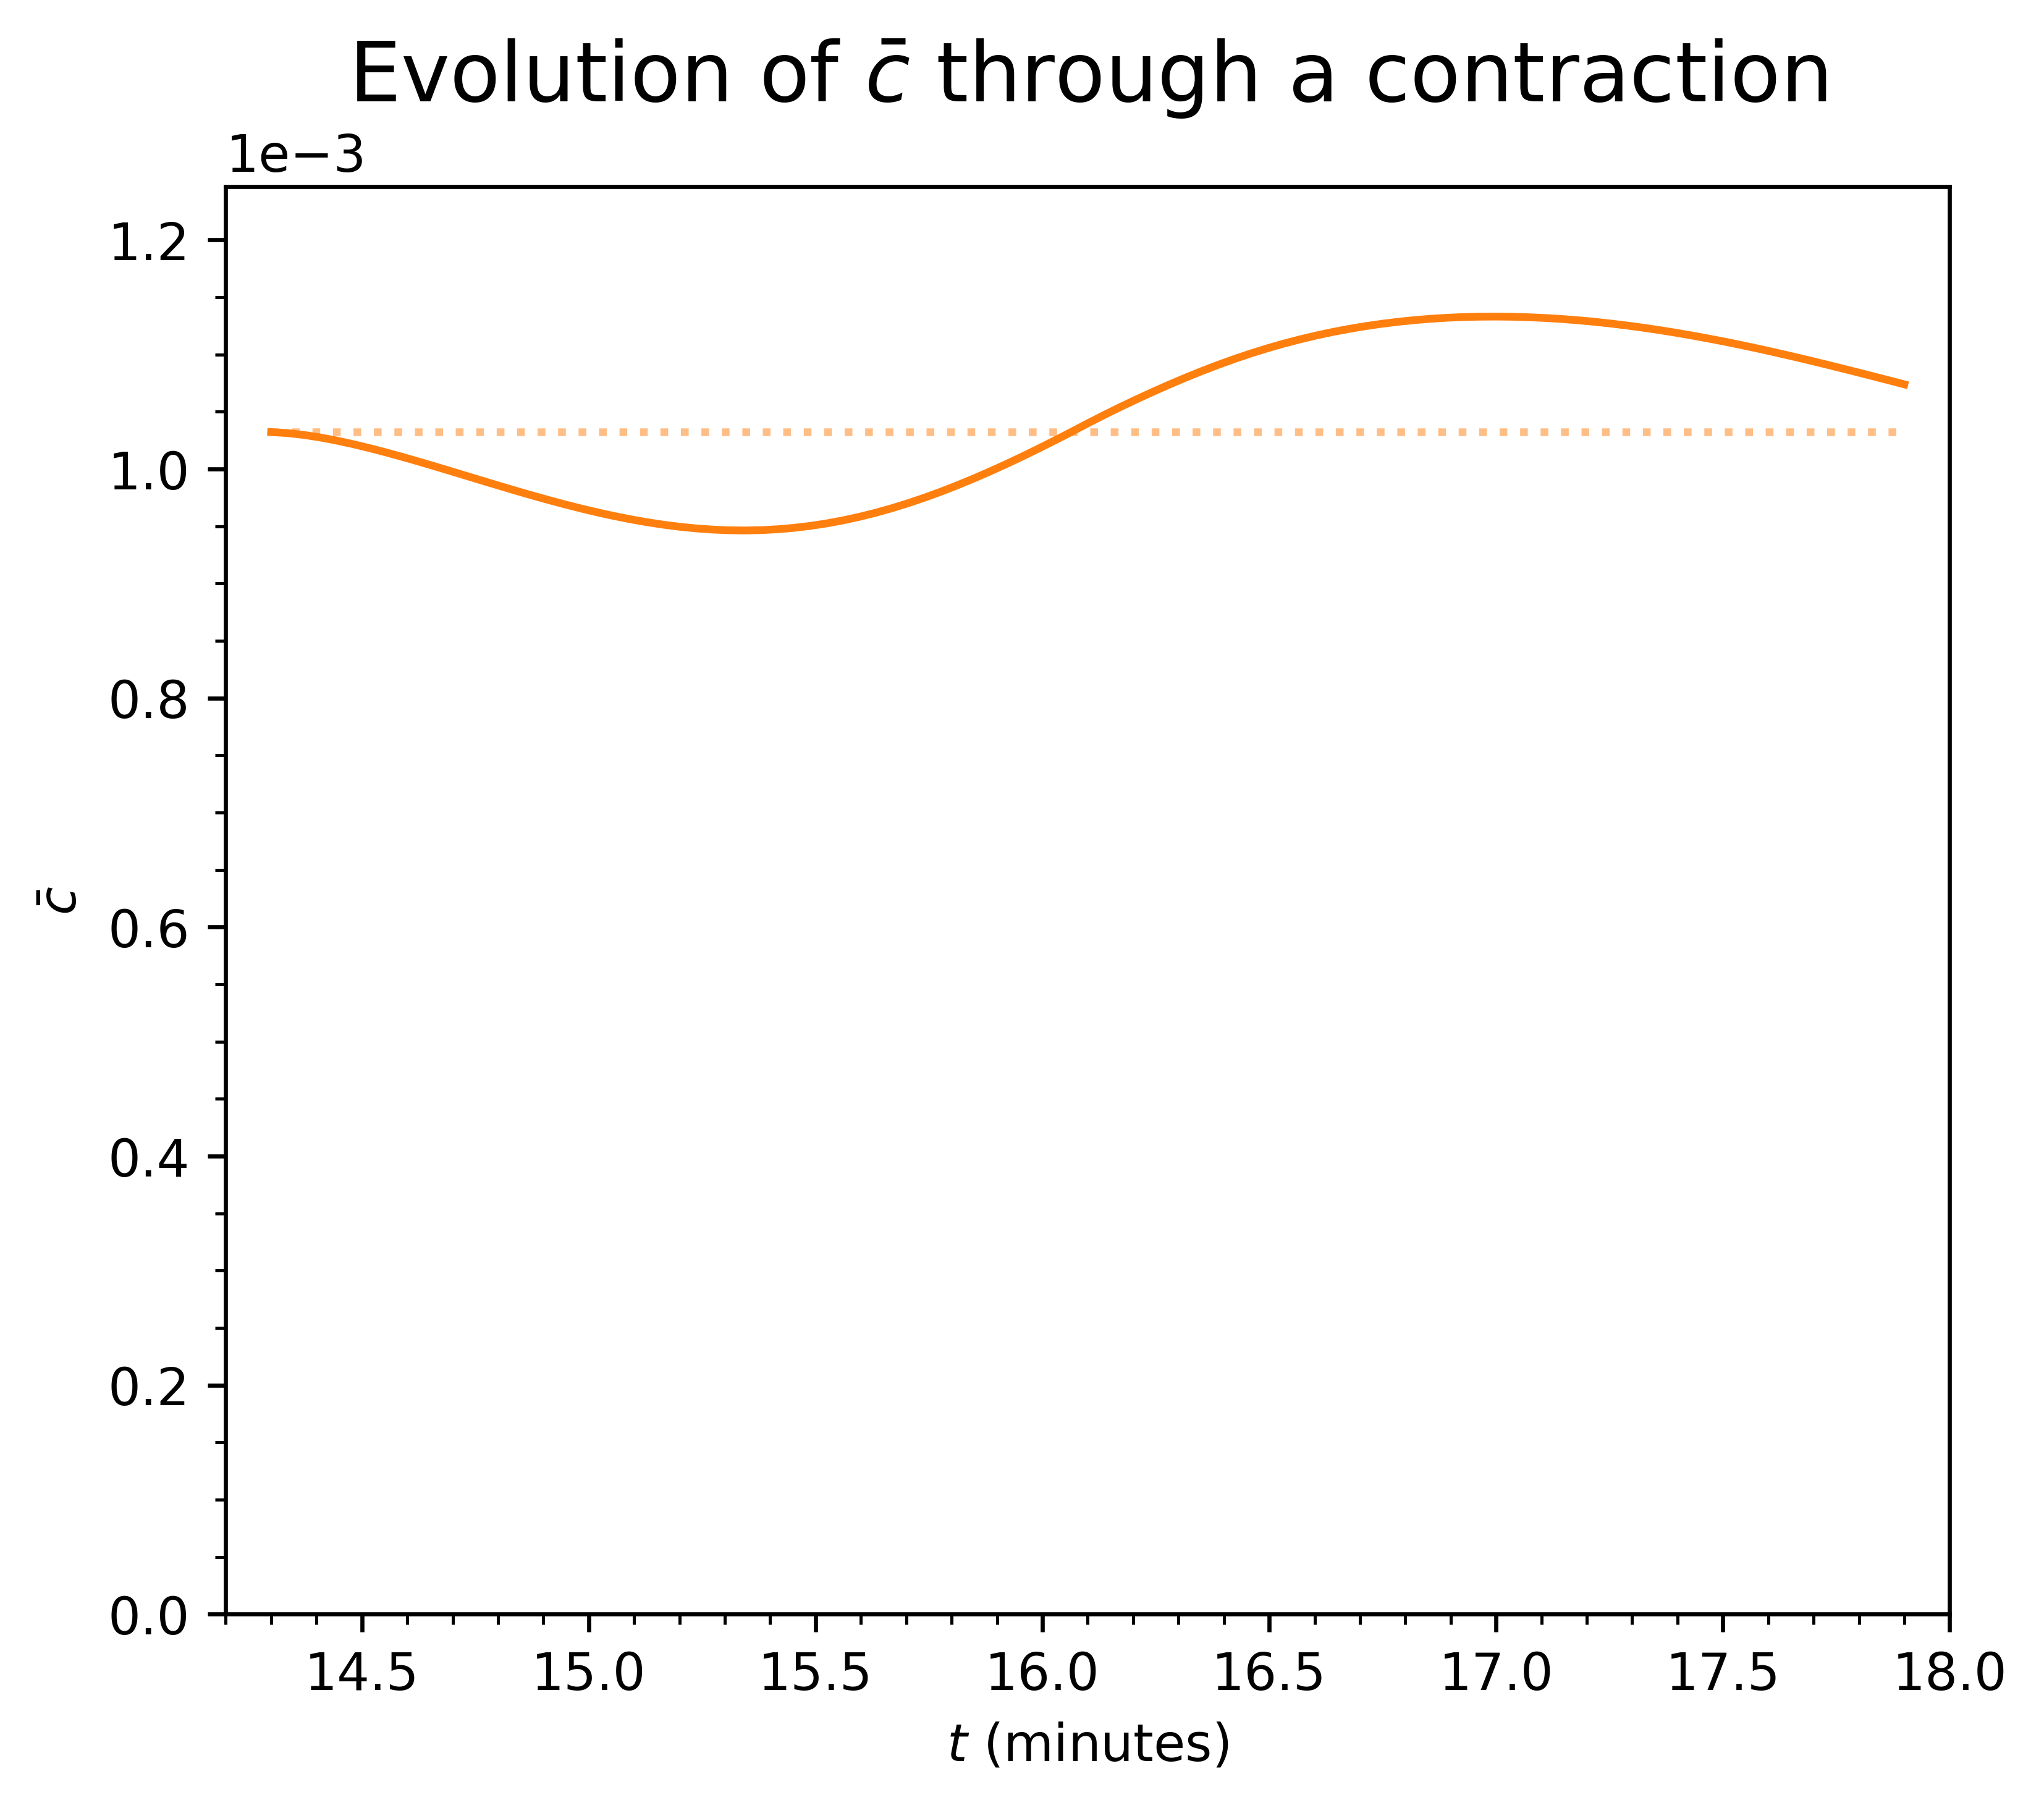
\includegraphics[width=\textwidth]{diagrams/results-contractions/mm-quantities-uptake.png}
                    \caption{}
                    \label{fig:mm-quantities:uptake}
                \end{subfigure}
                \caption{Graphs show how (a) $\bar{v}(\Omega)$ (Equation \eqref{eq:eff-v}) and (b) $\bar{c}$ (Equation \eqref{eq:eff-c}) vary throughout a contraction of the problem presented in \S\ref{sec:contractions:placenta}. Horizontal dotted lines indicate the value of these measures at time $t = T_0$.}
                \label{fig:mm-quantities}
            \end{figure}

            Figure \ref{fig:mm-quantities:velocity} shows that the average speed of the blood increases when the domain contracts, and decreases again when the domain expands. Interestingly, the peak of $\bar{v}(\Omega)$ corresponds to $t = \qty{15.9}{\minute}$, which is $\qty{0.2}{\minute}$ before the domain is at its smallest; as the domain velocity is decelerating toward this minimal domain size, this could be due to inertial effects on the blood which cause an augmented maximum. Likewise, there is a minimum $\qty{0.2}{\minute}$ before the maximum domain size is regained at $t = \qty{17.9}{\minute}$.
            
            Figure \ref{fig:mm-quantities:uptake} shows slightly different behaviour, where oxygen uptake is lowest during the period of most rapid contraction and highest during the period of most rapid expansion; these correspond to what we saw when visualising the oxygen concentration field in Figure \ref{fig:moving-mesh-placenta-transport:5}, where certain areas of the domain appeared to have lower oxygen concentration during the contraction and higher oxygen concentration during the expansion. The most significant feature of this graph is that the oxygen uptake is increased when the placenta returns to its original size at $t = \qty{17.9}{\minute}$, indicated by the solid line being higher than the dotted line. This simulation therefore supports the theory that placental contractions could assist maternal circulation by ejecting stagnant deoxygenated blood and improve oxygen delivery to the fetus \cite{dellschaftHaemodynamicsHumanPlacenta2020}.

            We will now close this chapter with some closing remarks, limitations of our contraction model, and suggested future work.

    \section{Summary} \label{sec:contractions:summary}
        In this chapter, we have introduced a basic model of prescribed boundary motion in order to investigate the effects of the recently-observed `utero-placental pump' contractions on maternal blood flow and oxygen transport dynamics. These are contractions that involve only the placenta and have been observed over $10$-minute intervals to periodically reduce placental volume by up to $40\%$ \cite{dellschaftHaemodynamicsHumanPlacenta2020}.

        In \S\ref{sec:contractions:dgfem-discretisation}, we used the Reynolds Transport Theorem to derive modified numerical methods for the flow and oxygen transport problem, which were valid on moving domains, and required minimal modification to the existing semilinear and bilinear forms of the discretisation. We then validated our numerical methods in \S\ref{sec:contractions:numerical-experiments} in two different ways: first, we used the method of manufactured solution (MMS) and showed that we obtain optimal spatial and temporal convergence rates under refinement; and secondly, we presented a physical problem where no-slip boundary conditions on an oscillating wall influence flow dynamics, which gave physically sensible flow dynamics.

        The main results of the chapter were presented in \S\ref{sec:contractions:placenta}, where we used volume information from MRI scan data to inform a domain velocity that represents a domain size change comparable to those found during a `utero-placental pump' contraction. Our results found that the blood flow field remained largely undisturbed, despite the relatively large domain size change; we noted that this is likely due to the long timescales upon which these contractions take place. We did, however, find that the oxygen concentration field was more visibly influenced by the boundary motion than the velocity field, with overall decreased oxygen uptake during the contracting phase and increased oxygen uptake during the expansion phase. Our simulation showed that contractions of this form do have an impact on oxygen concentration dynamics and oxygen uptake by the villous tree.

        For clarity, the model of the utero-placental pump we have presented here is highly simplified and does not consider the physical mechanisms driving the contractions. In particular, we have assumed a simple form for the domain velocity, and used this over a shorter \qty{3.6}{\minute} period covering the fastest volume change rate, rather than the full \qty{26}{\minute} presented in the data of \citeauthor{gowlandCharacterisingPlacentalContractions2024} \cite{gowlandCharacterisingPlacentalContractions2024}. Furthermore, the results of \citeauthor{dellschaftHaemodynamicsHumanPlacenta2020} \cite{dellschaftHaemodynamicsHumanPlacenta2020} show very little change in the thickness of the placenta between the chorionic and basal plates, with the contraction primarily taking place in the horizontal direction (when viewed in the orientation we have presented in this thesis); future work taking this approach could therefore simulate the entire contraction length and consider domain velocities that cause shape change only in the horizontal direction. Additionally, future studies could investigate the effect that villous tree density and shape has on flow dynamics and oxygen uptake.

        The cause of these contractions is currently unknown \cite{dellschaftHaemodynamicsHumanPlacenta2020}, but it is thought that they may be related to previous reports of contracted villous trees, which are sometimes anchored (i.e., connected) to the basal plate \cite{dellschaftHaemodynamicsHumanPlacenta2020,katoVillousTreeModel2017}. An interesting extension to this work would be to use the work of \citeauthor{katoVillousTreeModel2017} \cite{katoVillousTreeModel2017} in designing a model of the utero-placental pump that respects the data of \citeauthor{gowlandCharacterisingPlacentalContractions2024} \cite{gowlandCharacterisingPlacentalContractions2024}. An alternative modelling approach could reapply one of the works from the existing fluid-structure interaction literature (e.g., \cite{houNumericalMethodsFluidStructure2012,doneaArbitraryLagrangianEulerian2004,ricardodasilvaNumericalSimulationsFluidstructure2007,collisEffectiveEquationsGoverning2017,formaggiaCardiovascularMathematicsModeling2010}), where the mechanism of interaction between the maternal blood and surrounding contracting tissue could be modelled; this is rather than imposing a prescribed boundary motion like we have in this thesis. 

        The evolutionary role of the contractions is unknown, but it has been suggested that they assist maternal circulation by ejecting stagnant deoxygenated blood so that it may be replaced by freshly oxygenated blood \cite{dellschaftHaemodynamicsHumanPlacenta2020}. \citeauthor{dellschaftHaemodynamicsHumanPlacenta2020} \cite{dellschaftHaemodynamicsHumanPlacenta2020} have also suggested the possibility that these contractions may have a role to play in diseased placentas, with the shape of a healthy contracted placenta resembling the shape of a diseased placenta.

        We will now conclude this thesis with some conclusions and future work.